\documentclass{LULCSProject}
\usepackage{amsmath}
\usepackage{enumitem}
\usepackage{listings}
\usepackage{graphicx}
\usepackage{graphicx} % Required for inserting images
\usepackage{natbib}
\usepackage{amsmath}
\usepackage{todonotes}
\usepackage{caption}
\usepackage{subcaption}
\usepackage{tcolorbox}


\lstset{language=Java,
	basicstyle=\small,
	identifierstyle=\emph}

\newcommand{\tvect}[3] { \ensuremath{\Bigl(\negthinspace\begin{smallmatrix}#1\\#2\\#3\end{smallmatrix}\Bigr)}}
\newcommand{\twovect}[2] { \ensuremath{\left(\negthinspace\begin{smallmatrix}#1\\#2\end{smallmatrix}\right)}}


\title{Imperfections in Reaction Diffusion Simulations}
\author{Dennis Barzanoff}
\date{\today}
%\BSc % \MEng \BEng etc. 
\supervisor{James Stovold}

\wordcount{8542} % number of words in your report 

\lstdefinestyle{customc}{
  belowcaptionskip=1\baselineskip,
  breaklines=true,
  frame=L,
  xleftmargin=\parindent,
  language=C,
  showstringspaces=false,
  basicstyle=\footnotesize\ttfamily,
  keywordstyle=\bfseries\color{green!40!black},
  commentstyle=\itshape\color{purple!40!black},
  identifierstyle=\color{blue},
  stringstyle=\color{orange},
}


\abstract{The project aims to explore how changes in light imperfections impact the realism of a BZ simulation as it's scaled in size. The code is in Metal/GPU and runs experiments varying different simulation parameters that correspond to real-world changes, and then measures results. Changes in light were found to significantly impact the correct behaviour of BZ computer simulations and more advanced light management tools such as LED panels are required to scale large BZ circuits.}


\declaration{
\\[.5em]
I certify that the material contained in this dissertation is my own work and does not contain unreferenced or unacknowledged material. I also warrant that the above statement applies to the
implementation of the project and all associated documentation. Regarding the electronically
submitted work, I consent to this being stored electronically and copied for assessment purposes,
including the School's use of plagiarism detection systems in order to check the integrity of
assessed work.\\
I agree to my dissertation being placed in the public domain, with my name explicitly included
as the author of the work.\\
Name: Dennis Barzanoff\\
Date: \today
}

% \dedication{
%   If you want to dedicate to someone in particular
% }

\begin{document}

\maketitle

\pagenumbering{Roman}

%\tableofcontents

\listoffigures
\newpage
% \begingroup
% \let\clearpage\relax
\listoftables
%\endgroup

\newpage
\pagenumbering{arabic}

%%
%% include your chapters here
%%
\chapter{Introduction}
% here im supposed to motivate the whole thing and introduce the reader to the topic
% talk about the project as a whole
% talk about the structure of the project
% what am i planning to do
% what is the motivation
% goals

A chemical computer is a computer that uses chemistry to perform computations. It is a new field of research where rapid innovations have taken place in recent years.
The project as a whole aims to explore how diffierent imperfections impact the realism of a chemical computer simulation when it is transferred to the real environment. 
Imperfections, such as light and temperature changes are among the most significant factors that can have an effect on the correctness of the computer.

\section{Document Structure}
This project is structured in the following way:

\begin{itemize}
    \item \textbf{Introduction} introduces the project and its goals.
    \item \textbf{Background \& Literature Review} gives a comprehensive introduction to the concepts of chemical computing and reaction diffusion.
    \item \textbf{Design \& Implementation} gives a general overview of the tools and technologies used in the project, however each chapter will have its own section on the process of conducting measurements and calculations.
    \item \textbf{Results} contains the body of the dissertation, where different imperfections are explored and interesting conclusions are reached.
    \item \textbf{Conclusion \& Future Work} summarises the findings of the project and gives a direction for possible future work and enhancements.
\end{itemize}

\section{Motivation}
During the research for the project, it was found that there is a lot of reasearch in the field, some in simulations, others in real life (see Chapter \ref{ch:background-lit-review}). 
However, there is not much research in between the real-life chemical computers and the simulated ones, leaving many questions unanswered. These questions are covered in Section \ref{sec:goals}.
This project was born in an effort to bridge the gap between the two, and to explore how far off the simulations are from the real world.


\section{Project Goals}\label{sec:goals}
The project goals revolve around exploring different imperfections that impact simulation realism.

\subsection{Chemical Computer Size Limitations} \label{sec:computer-size}
Most chemical circuits in real life are done in a petri dish and simulations are done in a 2D grid that represents that petri dish.
It is unclear what impact the size of the petri dish has on the performace of the computer. Simulations do not take this into account and assume it works the same with any size. 
It is also unclear how to recreate a chemical computer from a simulation into a petri dish, namely, the size of the petri dish. 
This is because the petri dish computer is measured in mm, while the simulation is in pixels. Section \ref{sec:mapping-simulation-to-real-life} explores this.

\subsection{Investigating the Effects of Imperfections on Illumination Uniformity}
Chemical computing uses light to mould out circuits where the reactions can operate inside of a small petri dish. 
Most research \todo{ref} uses a constant light source in the form of a hallougen light bulb, but this light source is not perfect and does not provide constant illumination across the whole dish. \todo{ref image}
This is done in several sections because they depend on each other. 
\begin{enumerate}
    \item[(1)] \textbf{Establishing Computer Limits:} The limits of the computer are established in Section \ref{sec:finding-phi-min-max}.
    \item[(2)] \textbf{Calculating Light Source Position and Imperfections:} The position of the light source is calculated in Section \ref{sec:light-imperfections}, along with the imperfections that come with it.
\end{enumerate}

\subsection{Estimating the Maximum Size of the Chemical Computer}
The Chemical Computer is as big as the petri dish it resides in. It is interesting if there is a maximum size that the computer can be before it stops working and 
what limits the size of the computer. 
Using the information detailed in items (1) and (2), the maximum size of the computer is calculated in Section \ref{sec:computer-size-limitations}.

\subsection{Impact of Reflection And Refraction on Light Loss}
The OHP sheet discussed in section \ref{sec:ohp-impact} is normally unaffected by light angle because the light bulb shined across the petri dish is directly above it and the angle of the light is very close to 90 degrees.
However, as discussed in section \ref{sec:computer-size}, as the circuit is scaled in size, the angle of the light changes and the OHP sheet starts to not let all the light through as some of it reflects away.
This is discussed in Section \ref{sec:reflection-refraction}.

\subsection{Impact of OHP Sheet Thickness on Light Absorption} \label{sec:ohp-impact}
Chemical circuits done in a petri dish use a thin sheet of plastic to hold the circuit mask in place. Most of it is transparent except for the mask, 
which is opaque and allos for illumination to impact only the parts of the circuit that are needed to be passive during the reaction.
This is talked about in section \ref{sec:absorption}.

\chapter{Design \& Implementation}
The project experimented with Flutter for the initial simulation due to the benefits of pixel-level control and fast prototyping (see Figure \ref{fig:first-waves} for a preview of the first successful waves). However, the rendering was too slow for large chemical circuits, so the GPU was needed, for which, as of March 2024 Flutter still has no official support. A custom version of the newest engine was tested to expose experimental GPU APIs as detailed in \href{flutter.dev/go/impeller-dart}{flutter.dev/go/impeller-dart}.
That did not work, so the Metal library was used to compute the simulation on the GPU. 
The Metal library is a low-level, high-performance API for the GPU, and it was chosen for its ability to run on Apple devices, which are widely used in the scientific community, the execution graph for the simulation is illustrated in Figure \ref{fig:metal-dependency-pipline}.
The implementation is done using two buffers and two CPU threads.
While the compute thread is computing the next state of the simulation by sending commands to the GPU,
the render thread is displaying the current state of the simulation on the screen.
The CPU has no knowledge of the state of the simulation and the assets used stay solely on the GPU, both 
during computation and during rendering. This allows for very high performance that is possible only because
of the fact that there is no copying of data between the CPU and the GPU aside from simple buffers used for communication.


\begin{figure}
    \centering
    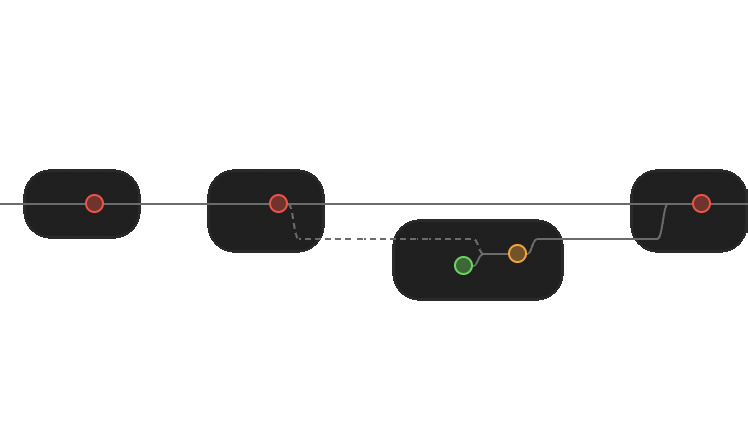
\includegraphics[width=0.5\linewidth]{metal-pipeline.png}
    \caption{The Metal Dependency Pipeline consists of a Compute Command Encoder (represented by red circles) and a Render Command Encoder (depicted by yellow circles). The Compute Command Encoder is run multiple times, performing as many calculations as possible. Simultaneously, the Render Command Encoder operates periodically to render the computed results. These two encoders work in parallel, with the Render Command Encoder producing output every time it gets a chance, while the Compute Command Encoder continuously performs computations most of the time.}
    \label{fig:metal-dependency-pipline}
\end{figure}

Conducting measurements was implemented using a sampling shader, which runs on the GPU, it is given a coordinate and returns information
back to the CPU. This is desyncrhonised from the computation of the simulation because it does not run on the compute thread.
Another more efficient and accurate way to measure is to add the measurement buffers directly to the compute shader.
That would allow for the measurement to happen at the same time and could also track the simulation time steps,
which is something that is not easy with the current implementation. 


The mathematical principles in the Oregonator model are described in section \ref{sec:oregonator-math}.
The parameters for the simulation are listed under table \ref{tab:simulation-parameters}. 
They are standard values widely used in the literature that experiments with the Oregonator model.
What each of them does is described in Chapter \ref{ch:introduction}.



\begin{table}
    \centering
    \begin{tabularx}{\textwidth}{|X|X|} 
        \hline
    \textbf{Parameter} & \textbf{Value} \\ \hline
    $\epsilon$         & 0.0243         \\
    $f$                & 1.4            \\ 
    $\phi_{\text{active}}$ & 0.054          \\ 
    $\phi_{\text{passive}}$ & 0.0975          \\
    $q$                & 0.002          \\ 
    $D_u$              & 0.45           \\ 
    $\Delta t$         & 0.001          \\
    $\Delta x$              & 0.25           \\
    \hline
    \end{tabularx}
    \caption{Simulation parameters with their respective values.}
    \label{tab:simulation-parameters}
\end{table}


\include{chapters/background-lit-review}
\chapter{Results}
This chapter aims to explore the operational boundaries of the chemical components in a Petri dish environment, focusing on the size limitations of the coincidence detector and the light sensitivity of a chemical diode.
A coincidence detector is crucial in the design of chemical circuits because it allows for an implementation of AND gates,
which are important for computing. This detector is illustrated in Figure \ref{fig:and-gate} and it works by having two waves come together from left and right and if they meet, they form a new wave that passes through the detector at the bottom.

The main objectives of the experiments are to find out the bounds and limitations of different chemical components in order to determine the feasibility of using them in a real-world environment.

\section{Mapping the Simulation Size to Real Life} \label{sec:mapping-simulation-to-real-life}
In order to understand how real light affects the chemical circuit, what needs to be established is the resolution of the circuit in real life and how it relates to the size of the detector. \cite{gorecki2003chemical} have recreated the circuit in a Petri dish, so we can use the size of the circuit in the Petri dish to map it to the size of the circuit in the simulation.
The goal here is to find a way to measure the size of the coincidence detector in real life, for which there is currently no data. The size of the coincidence detector is crucial for the design of the Petri dish, as it determines the minimum size of the Petri dish required to accommodate the detector. 

In order to measure that, the coincidence detector had to be designed first and that is covered in Appendix~\ref{chap:creating-detector}, the final component is illustrated in Figure \ref{fig:and-gate}.


\begin{figure}
    \centering
    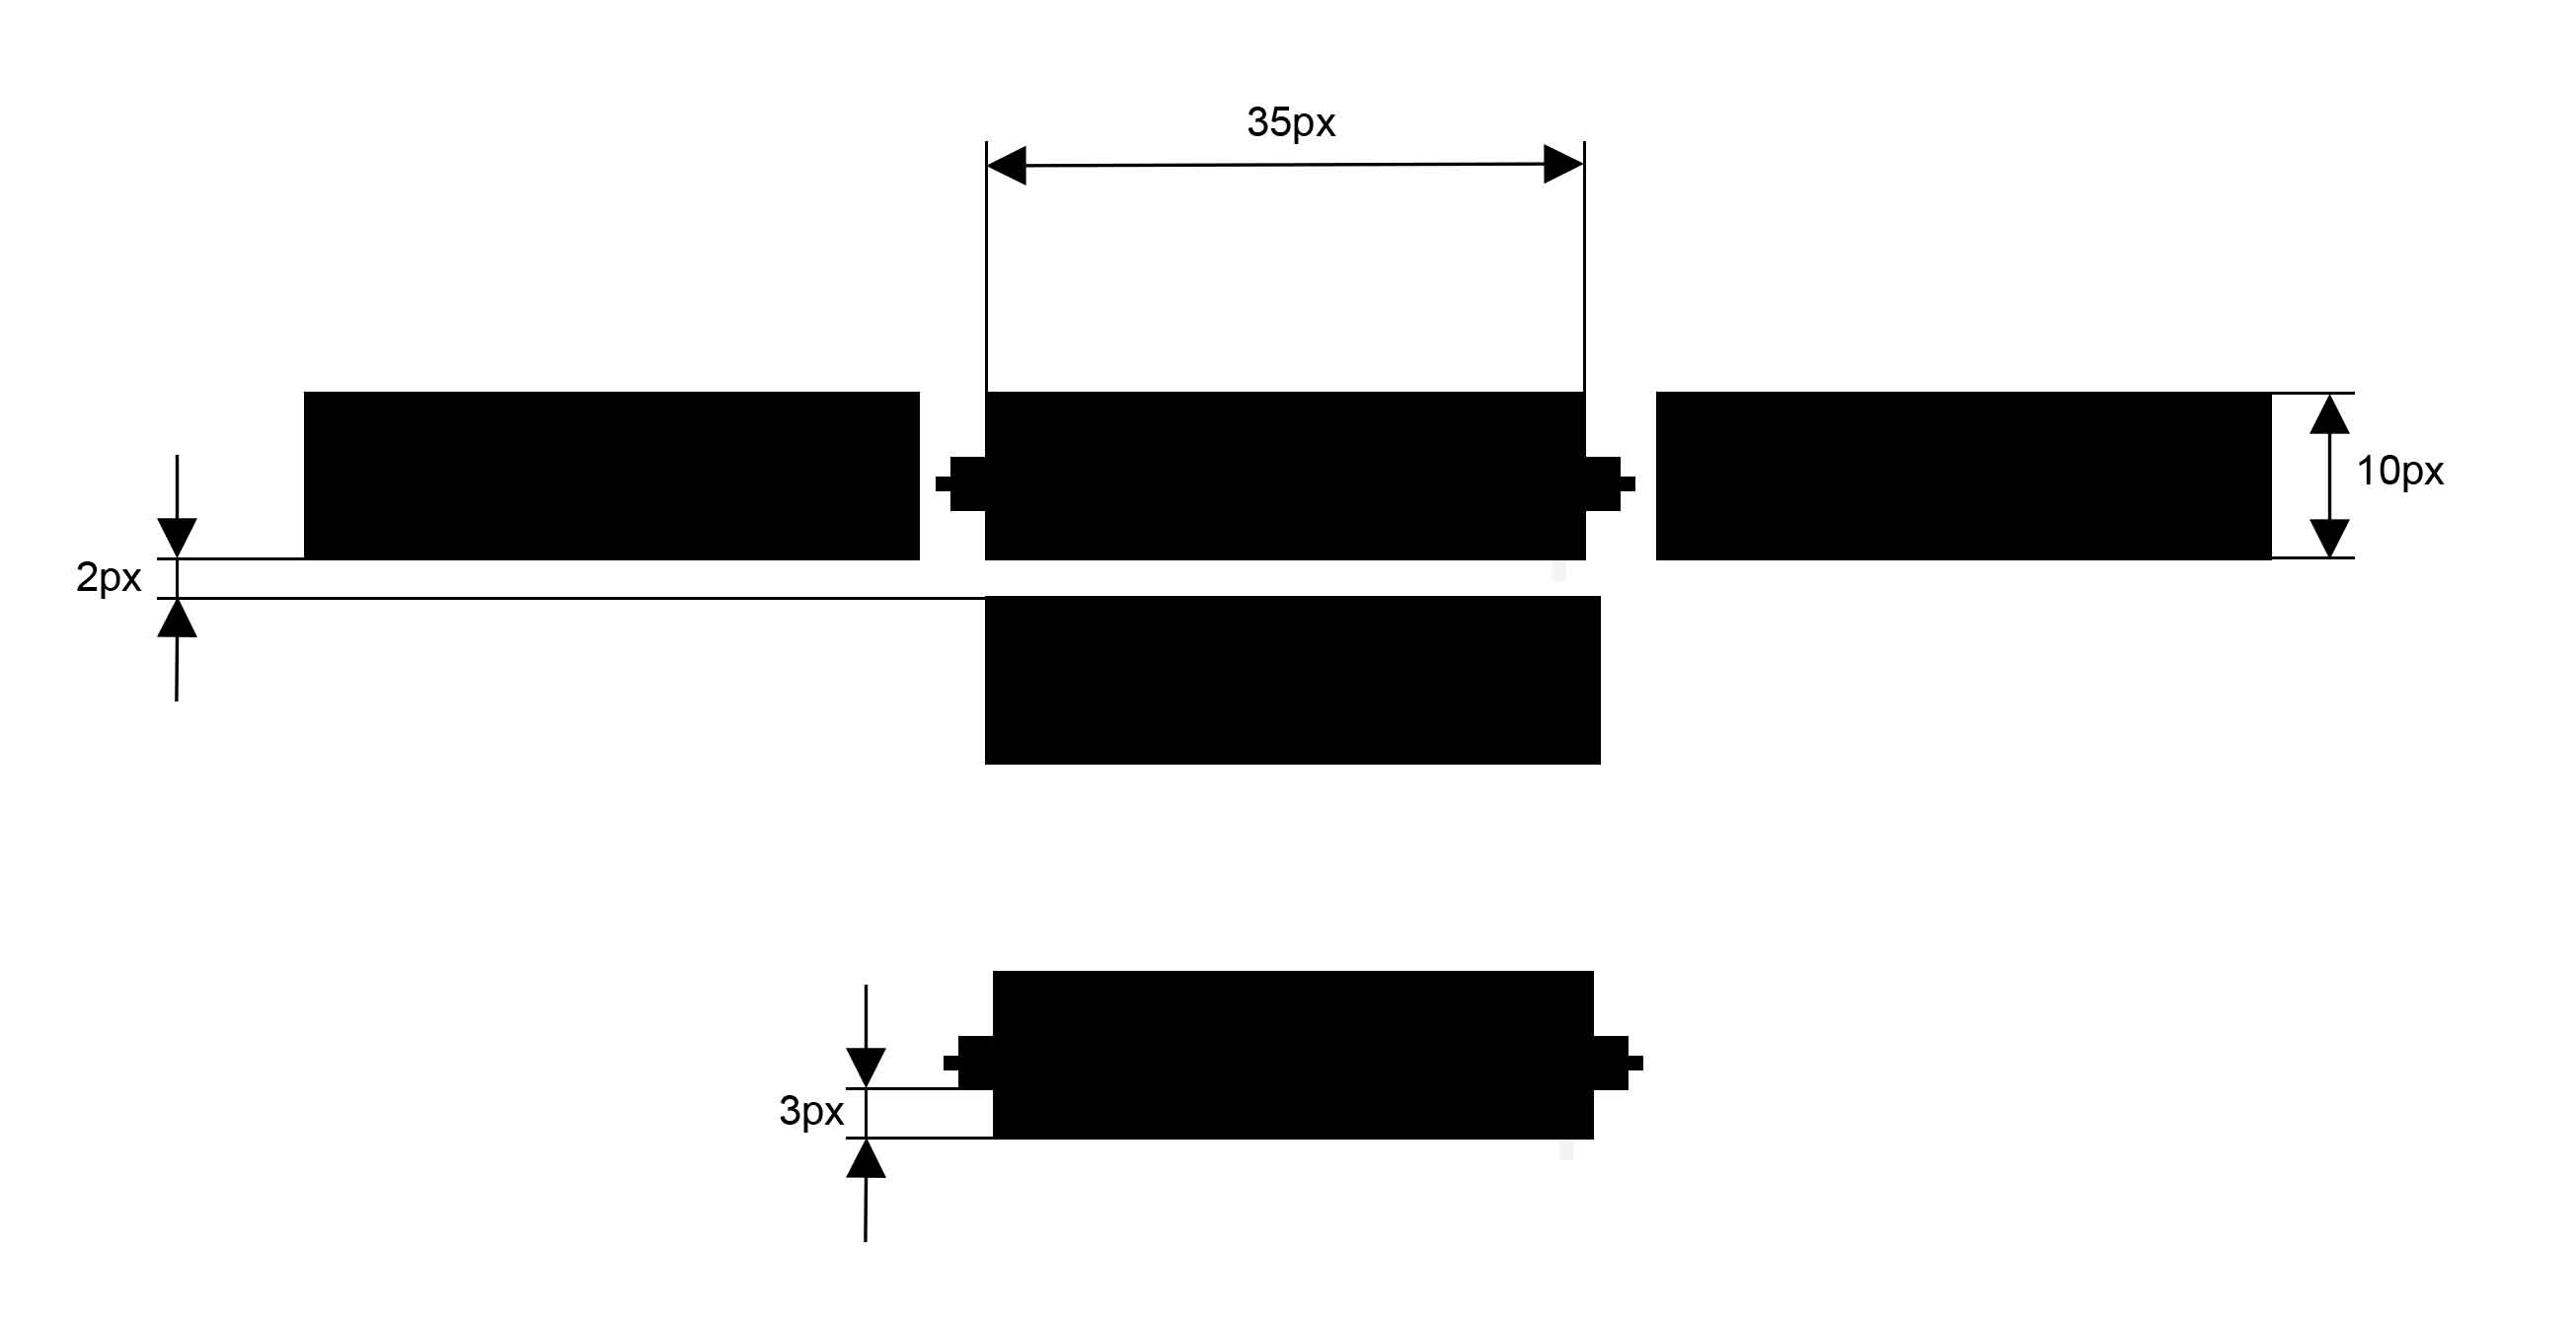
\includegraphics[width=1\linewidth]{measurement-and.jpg}
    \caption{First working AND gate}
    \label{fig:and-gate}
\end{figure}

The design of the detector (Fig. \ref{fig:and-gate}) implies that there is no max size for the length of the coincidence medium in the detector circuit as the waves have a width equal to the width of the coincidence channel.
\begin{tcolorbox}[colback=red!5!white,colframe=red!75!black,title=Assumption]
    The size of the Petri dish is \textbf{assumed} to be unsubstantially larger than the size of the chemical circuit inside of it. Continuing from both sizes are referred to interchangeably.
\end{tcolorbox}
A significant milestone in the practical application of chemical computing was achieved through the real-life implementation of an AND gate using the Belousov-Zhabotinsky (BZ) reaction. This implementation, detailed by \cite{gorecki2003chemical} and shown in Figure \ref{fig:bz-and-gate}, serves as a cornerstone example of how chemical reactions can be harnessed for computational purposes.

\begin{figure}
    \centering
    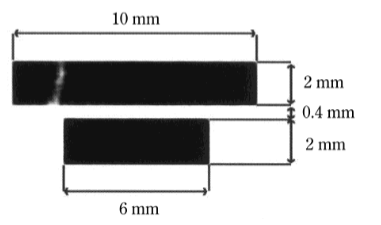
\includegraphics[width=0.6\linewidth]{images/Screenshot 2024-03-10 at 20.59.51.png}
    \caption{Real-life AND gate using BZ reaction \citep{gorecki2003chemical}}
    \label{fig:bz-and-gate}
\end{figure}


Now, this is just a simulation we are doing, so to get the mapping for a real Petri dish, we can use the dimentions of the gate in a Petri dish. 
In \cite{gorecki2003chemical}, the exact dimensions in mm of the collision detector, signal channel of 10cm, and a membrane filter of 2.5cm inside of the Petri dish are specified. These dimensions can be used to map it to the one in our simulation.


Given the following mapping from real life measurements to simulation pixels:
\begin{itemize}
    \item Stripe width: \(2 \text{ mm} = 10 \text{ px}\)
    \item Channel gap: \(0.4 \text{ mm} = 2 \text{ px}\)
\end{itemize}

We can establish a scaling factor for the conversion from millimeters to pixels.
For the stripe width:
\[ \text{Scaling factor} = \frac{10 \text{ px}}{2 \text{ mm}} = 5 \text{ px/mm} \]

For the channel gap:
\[ \text{Scaling factor} = \frac{2 \text{ px}}{0.4 \text{ mm}} = \frac{2 \text{ px}}{\frac{2}{5} \text{ mm}} = 5 \text{ px/mm} \]

Thus, both measurements confirm the same scaling factor. Using this consistent scaling factor, we can convert any measurement from millimeters to pixels.

Using this scaling factor, we can convert any measurement from millimeters to pixels.
For a dimension of \(10 \text{ mm} \times 4.4 \text{ mm}\), the conversion would be:

\begin{align*}
\text{Width in pixels} &= 10 \text{ mm} \times 5 \text{ px/mm} = 50 \text{ px} \\
\text{Height in pixels} &= 4.4 \text{ mm} \times 5 \text{ px/mm} = 22 \text{ px}
\end{align*}

Thus, a real-life size of \(10 \text{ mm} \times 4.4 \text{ mm}\) would map to a size of \(50 \text{ px} \times 22 \text{ px}\) in the simulation.
More importantly, the simulation uses details as small as $1\text{px}^2$, which would amount to $\frac{1}{5}\text{mm}^2$ in real life, which would be infeasible because details smaller than $1\text{mm}^2$ are difficult to control accurately.
This means we would need to scale the simulation up in order to have details easier to control. 
However, as we scale it up, the surface area of the Petri dish becomes larger and the angle of incidence of the light becomes more significant, which is a problem we will explore later on in section \ref{sec:light-imperfections}.
The reason there is a section before that is because 


\section{Finding $\phi_{\text{min}}$ and $\phi_{\text{max}}$ for a Chemical Diode} \label{sec:finding-phi-min-max}
As mentioned in equation \ref{eq:u-partial-t}, $\phi$ is external illumination that creates the chemical circuit. It sets the value of $\phi$ to either $\phi_{\text{active}}$ or $\phi_{\text{passive}}$. 
$\phi$ values control the lighting conditions of the chemical circuit.
Active regions are where it is dark/unilluminated and passive regions are where there is light/illlumination.
The reason behind the need to measure the $\phi$ values for a Chemical Diode stems from the fact that a chemical diode is less sensitive to changes in $\phi$ values than other chemical components.
This means that the diode can still operate even outside the values for $\phi$ established in literature. In order to see where chemical computers break, we need to measure each component and see where it breaks.
The operational range for a whole computer is the intersection of the operational ranges of every component, which is equal to that of the most sensitive performing component.
Here $\phi_{\text{passive}}$ is measured at different values because that is the value controlling the illuminated area, which makes the circuit there ``passive''. This simulates less illumination of light at the diode, altering its behaviour.
\subsection{Measuring $\phi_{\text{min}}$, $\phi_{\text{max}}$}


During the evaluation of $\phi_{\text{min}}$, $\phi_{\text{max}}$, the diode had to be tested from numerous directions to determine the minimum and maximum values of $\phi_{\text{passive}}$ where it still functions correctly as a diode, 
which means that it passes waves from right to left, but never from left to right. As we approach the limits, new cases start appearing where the wave becomes able to pass through from a very specific angle that changes as we change the phi value, 
making it impossible to automatically test, so manual testing was needed to verify if the diode works in every single use case for the limit phi values. Also, the minimum and maximum values start to highly depend on the testing conditions, 
and whether the diode works or not starts to depend on how you are using it; for example, do you start a wave right at the diode? 
If not, what is the minimum distance the diode has to work for? This greatly changes the minimum and maximum phi values. 
\subsubsection*{Measurement Methodology}
The measurement was done by starting a wave at a distance from the diode and measuring if it passes through the diode. 
it's done from both directions.
tested from multiple angles and distances and qualitatively assessed if it still performs as a diode under every single case.
The investigation is trying to establish $\phi_{\text{min}}$ and $\phi_{\text{max}}$ for the diode, which are the operational boundaries for the $\phi_{\text{passive}}$ values that the diode can tolerate, 
which represent the less than ideal lighting conditions are are trying to explore.
we know that the diode operates mostly at $\phi_{\text{passive} = \phi_{\text{literature}}} = 0.0975$. 
We start from this value and start going in both directions, increasing and decreasing the value of $\phi_{\text{passive}}$ and measuring if the diode still works.
$\phi_{\text{current}} = \phi_{\text{literature}} = 0.0975$
\begin{algorithm}
    \caption{Detailed $\phi$ Exploration Algorithm. It works by starting from $\phi_{\text{literature}}$ and searching for the last value where the diode still works. 
    The function \text{TestDiode} returns true if the diode works and false if it does not. This is done manually by performing comprehensive tests on the diode from both directions. 
    It should let the wave through from right to left, but never from left to right. This shall be true for all angles and distances.
    The whole algorithm is run manually and is written out here just for illustrative purposes.}
    \label{alg:phi-exploration}
    \begin{algorithmic}[1]
        \State $\phi_{\text{current}} \leftarrow \phi_{\text{literature}}$
        \State $precision \leftarrow 0.5$ \Comment{Starting precision}
        \State $step \leftarrow 0.05$ \Comment{Initial step size}
        \While{$precision \geq 0.0001$} \Comment{Continue until precision is fine enough}
            \State $found \leftarrow$ \textbf{false}
            \While{\textbf{not} $found$}
                \If{\text{TestDiode}($\phi_{\text{current}} + step$)}
                    \State $\phi_{\text{current}} \leftarrow \phi_{\text{current}} + step$
                \ElsIf{\text{TestDiode}($\phi_{\text{current}} - step$)}
                    \State $\phi_{\text{current}} \leftarrow \phi_{\text{current}} - step$
                \Else
                    \State $found \leftarrow$ \textbf{true}
                \EndIf
            \EndWhile
            \State $precision \leftarrow precision / 10$ \Comment{Increase precision}
            \State $step \leftarrow 0.5 * precision$ \Comment{Adjust step size based on new precision}
        \EndWhile
        \State $\phi_{\text{functional}} \leftarrow \phi_{\text{current}}$
    \end{algorithmic}
\end{algorithm}


Algorithm \ref{alg:phi-exploration} outlines the process of finding the boundaries of $\phi_{\text{passive}}$ for the diode. It is run twice, 
once with \verb|step=0.05| and once with \verb|step=-0.05| to go in the other direction.

\subsubsection*{Results}

Results of measurement: 
\begin{itemize}
    \item $\phi_{\text{max}} = 0.106127$
    \item $\phi_{\text{min}} = 0.09555$
\end{itemize}

That is, as long as $\phi_{\text{min}} < \phi_{\text{passive}} < \phi_{\text{max}}$, then the diode will function as expected, even though the propagation time would still be affected (as seen in Figure \ref{fig:phi_passive_propagation_times}), causing synchronisation problems in larger circuits.


\subsection{Propagation Time Variation of the Diode Under Different Lighting Conditions}\label{sec:propagation-time-variation}
The reason we are looking at propagation time varyiation is because if that changes in response to the lighting conditions,
then the diode will behave as expected, but larger circuits that synchronise with the output of that diode and other chemical components
will be affected by this change and might not work as expected.
\subsubsection*{Methodology}
The way the experiment was set up was that a diode was set up in Figure \ref{fig:diode_experiment} where a wave was launched 25 px from the diode to allow it to pass through the diode and reach a small white flag where the wave is expected and the experiments are evaluated. A step in the diagram means one simulation pass. The parameters of the experiment were the following:
\begin{itemize}
    \item Number of $\phi_{\text{passive}}$ values: 30, of which only 19 succeeded, the remaining 11 could not pass through the diode due to the parameter being too out of range.
    \item Interval size: 0.0013448276
    \item Number of runs per $\phi_{\text{passive}}$ values: 7
    \item $\phi_{\text{start}}$: 0.08066608
    \item $\phi_{\text{end}}$: 0.121010914, never reached because once a wave passes through the diode, the concentration no longer reaches zero fully and that leaves a very small amount of inhibitor at the diode and due to the borderline value of $\phi_{\text{passive}}$ the next waves never manage to penetrate to get measured, so the highest measured value for $\phi_{\text{passive}}$ is 0.10487298
    \item Wave start: 39px before diode, which was observed to be enough to allow for the proper formation of the wave
    such that it can pass through the diode.
    \item Wave measure: 31px after diode, which was far away enough to measure a fully formed wave, provided
    that one passed through the diode. 
    \item $dt$: 0.001, also serves as a reference point for the amount of steps.
    \item Measurement interval: about every 5 steps, depending on the GPU frame rendering schedule
\end{itemize}

It is possible to run the experiment much more accurately, eliminating the need for multiple runs for the same $\phi_{\text{passive}}$ value we measured at every step and did not simulate another step in the simulation until the measurement was complete. However, that would drastically slow down the experiment, making it run for hours instead of minutes. For the purposes of merely showing that the propagation changes along with the slope, it was enough accuracy, so the faster and more inaccurate solution was chosen.

\begin{figure}
    \centering
    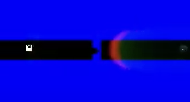
\includegraphics[width=0.5\linewidth]{diode.png}
    \caption{Diode Experiment}
    \label{fig:diode_experiment}
\end{figure}

So, the following limitation were found while working with the simulation. Due to the act that in metal sampling is a rendering operation, it cannot be done during the computation of the simulation. That means that I would have to synchronise it to run with rendering speed, but that would make the simulation too slow to run many experiments. It uses the step speed of the simulation, 1 frame = about 150 steps in the simulation. This is still accurate enough. I ran at $dt=0.001$.
To get better results the computation was run at $dt=0.001$ was done every 300 microseconds.
Additional values were added in between $\phi_{\text{min}}$ and $\phi_{\text{max}}$ where the curve started to change, and the results can be seen in Figure \ref{fig:phi_passive_propagation_times_detail_max}.

\subsection{Results}

The results of the experiment can be seen in Figure \ref{fig:phi_passive_propagation_times}. The propagation time decreases as there is less light, indicated by the decrease in the value of $\phi_{\text{passive}}$ and the reverse. This is to be expected, as a lower value brings it closer to $\phi_{\text{active}}$ (darkness), and illumination is an inhibitor. 
The reason the circuit has a higher tolerance to less light, compared to more light, is because the diode is much more resistant in the reverse direction as the wave has to go through a reverse triangle, 
which is specifically made to stop the propagation of waves. 
The diode also has a high tolerance to $\phi_{\text{passive}}$ increasing due to an additional spike added to the diode, which helps weaves to cross the gap easier, even when there is more light. The reason for $\phi_{\text{max}} < \phi_{\text{end}}$, meaning the diode was still letting the wave through left to right and not right to left at $\phi_{end}$, but it was not at other angles when tested, so the experiment measured propagation time, but the diode was only partially functional at these values

\begin{figure}
    \centering
    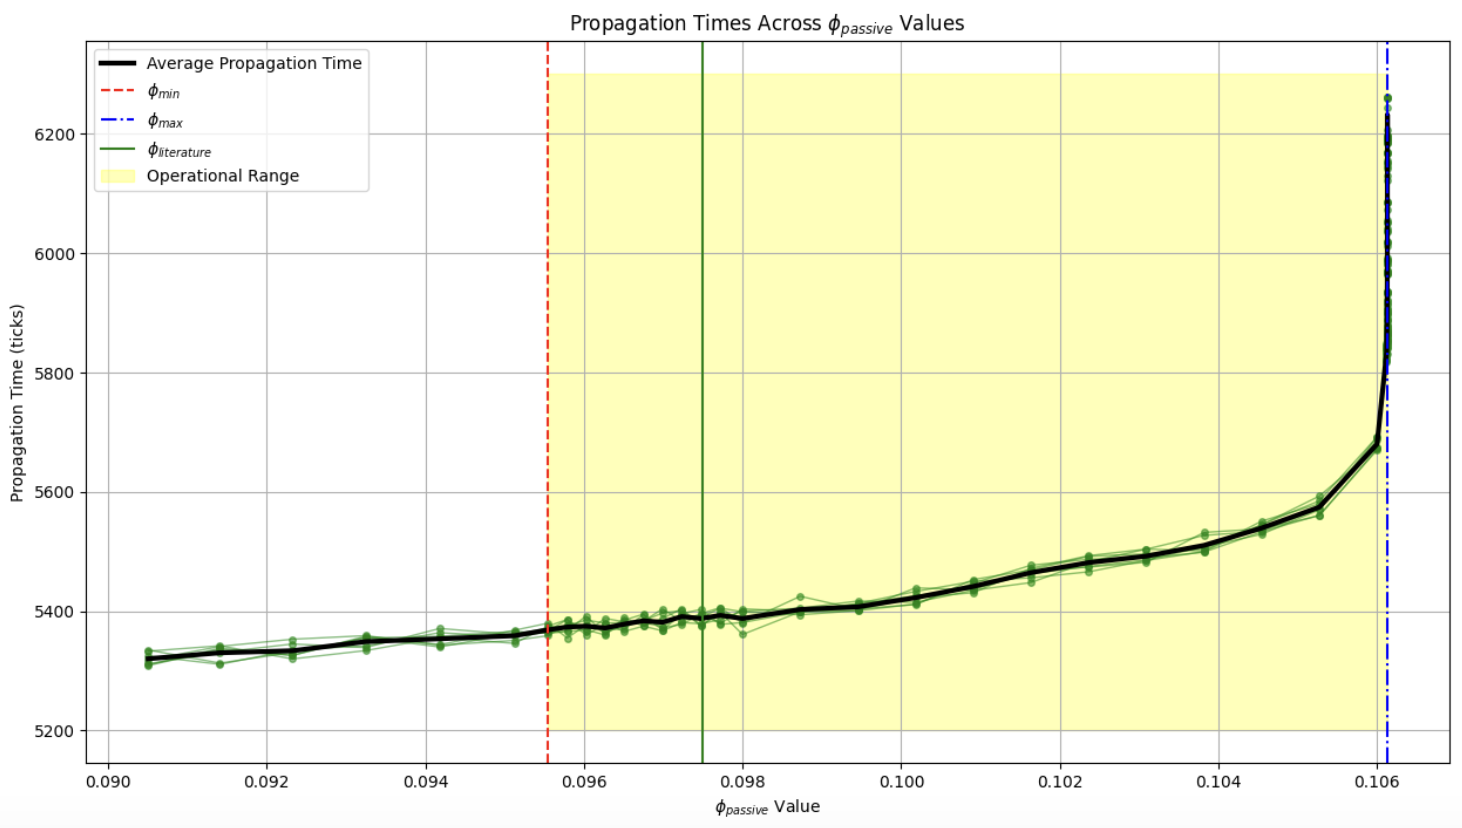
\includegraphics[width=\linewidth]{Screenshot 2024-03-09 at 10.35.01.png}
    \caption{Propagation times for various $\phi_{\text{passive}}$ values within the limits of $\phi_{\text{min}}$ and $\phi_{\text{max}}$, 
    illustrating the experimental outcomes of testing a diode in a Belousov-Zhabotinsky reaction. 
    Each point represents a propagation time measurement for a given $\phi_{\text{passive}}$, 
    with the average propagation time across measurements shown by a thicker black line. 
    The shaded area between $\phi_{\text{min}}$ (red dashed line) and $\phi_{\text{max}}$ (blue dashed line) highlights the range 
    where the diode works correctly, with the $\phi$ used commonly in literature marked by a solid green line.}
    \label{fig:phi_passive_propagation_times}
    
\end{figure}

\begin{figure}
    \centering
    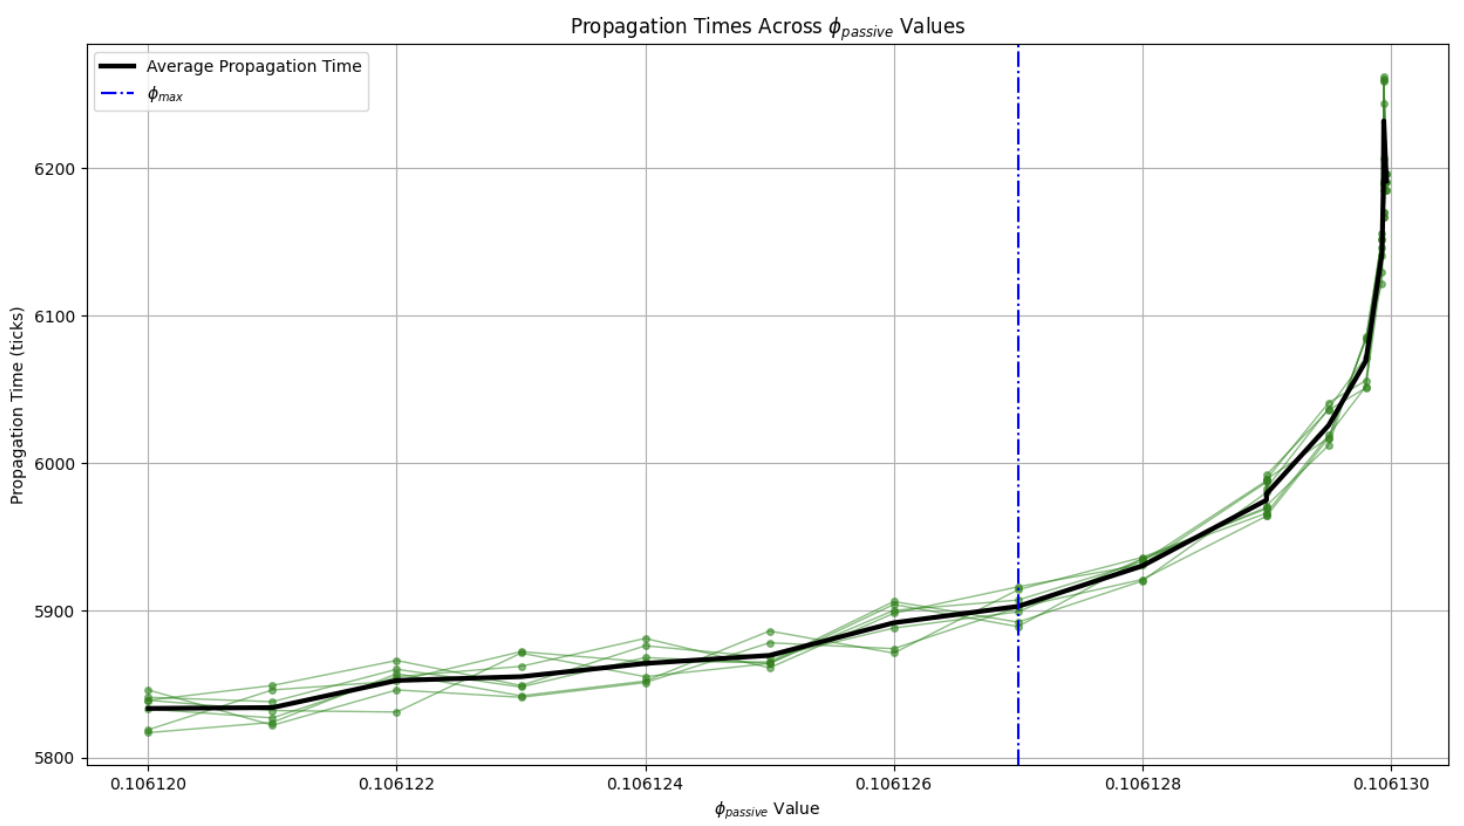
\includegraphics[width=1\linewidth]{Screenshot 2024-03-10 at 07.50.59.png}
    \caption{Propagation times around the value of $\phi_{\text{max}}$. The range of $\phi$ is $\phi_{\text{max}} - 7 \times 10^{-6} \leq \phi \leq \phi_{\text{max}} + 3 \times 10^{-6}$}
    \label{fig:phi_passive_propagation_times_detail_max}
\end{figure}



\begin{figure}
	\centering
	\begin{subfigure}{0.24\textwidth}
		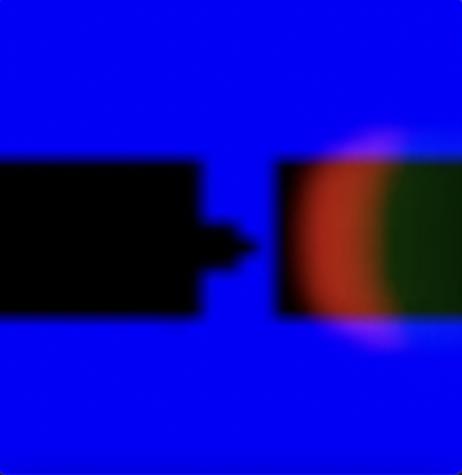
\includegraphics[width=\linewidth]{diode/easy/Screenshot 2024-03-09 at 16.21.56.png}
		\caption*{$t = 1$}
	\end{subfigure}
	\begin{subfigure}{0.24\textwidth}
		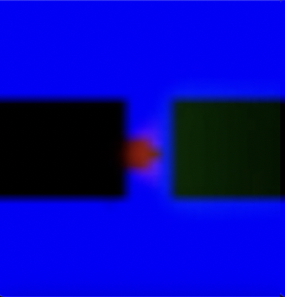
\includegraphics[width=\linewidth]{diode/easy/Screenshot 2024-03-09 at 16.22.24.png}
		\caption*{$t = 2$}
	\end{subfigure}
    \begin{subfigure}{0.24\textwidth}
		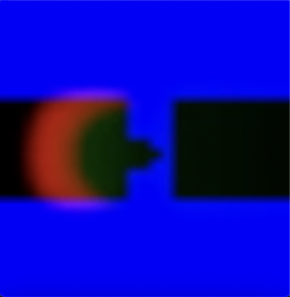
\includegraphics[width=\linewidth]{diode/easy/Screenshot 2024-03-09 at 16.22.35.png}
		\caption*{$t = 3$}
	\end{subfigure}
    \begin{subfigure}{0.24\textwidth}
		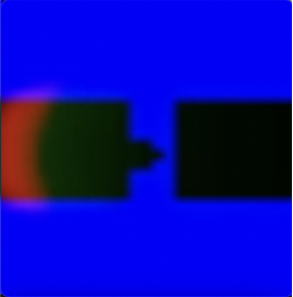
\includegraphics[width=\linewidth]{diode/easy/Screenshot 2024-03-09 at 16.22.45.png}
		\caption*{$t = 4$}
	\end{subfigure}

	\begin{subfigure}{0.24\textwidth}
		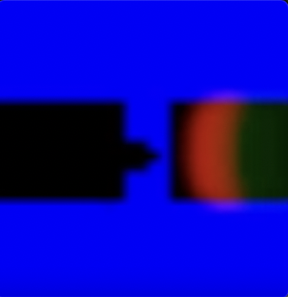
\includegraphics[width=\linewidth]{diode/hard/Screenshot 2024-03-09 at 16.23.41.png}
		\caption*{$t = 1$}
	\end{subfigure}
	\begin{subfigure}{0.24\textwidth}
		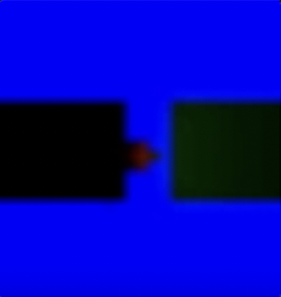
\includegraphics[width=\linewidth]{diode/hard/Screenshot 2024-03-09 at 16.23.48.png}
		\caption*{$t = 2$}
	\end{subfigure}
    \begin{subfigure}{0.24\textwidth}
		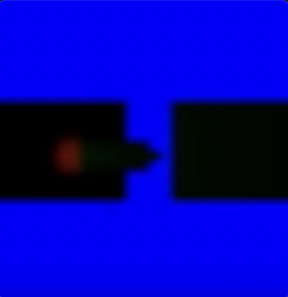
\includegraphics[width=\linewidth]{diode/hard/Screenshot 2024-03-09 at 16.23.55.png}
		\caption*{$t = 3$}
	\end{subfigure}
    \begin{subfigure}{0.24\textwidth}
		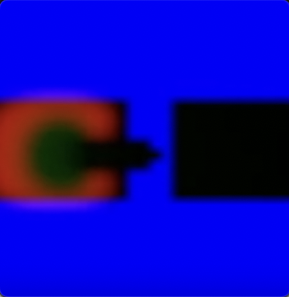
\includegraphics[width=\linewidth]{diode/hard/Screenshot 2024-03-09 at 16.24.01.png}
		\caption*{$t = 4$}
	\end{subfigure}

	\caption{Comparison of two waves passing through a diode. Above $\phi_{\text{passive}} = \phi_{\text{literature}}$, below $\phi_{\text{passive}} = \phi_{max}$. Both have different propagation speeds, so they have been equalised for the purpose of comparing their interaction with the diode side by side. The second wave takes substantially more time to form and is about 700 time steps slower as seen in Figure \ref{fig:phi_passive_propagation_times_detail_max}, which is quite a lot in such simulations.}
	\label{fig:comparison_diode}
\end{figure}

% \section{Calculating Possible Movement of the Light Source}
\section{Estimating The Light Source's Position}\label{sec:light-imperfections}



Identifying the minimal operational conditions for the AND gate in real life involves examining light intensity, angle of incidence, and the effect of the thickness of the beam of light on the BZ reaction.


Some circuits \todo{is it the same reaction} can be influenced by temperature, such as \cite{yamada2022artificial}, which uses a more complex model of the oregonator.  .


Shining light on the BZ surface: \citep{barry1979methods}
The catalyst in these reactions is light, using light we can modulate the speed using $\Phi$.
A light bulb is shined over the Petri dish (fig. \ref{fig:light-over-petri})

Given multiple light sources, the total illumination $I_{\text{total}}$ at a point on a surface is the sum of the illuminations from each individual light source (fig. \ref{fig:light-flux-petri-dish}). The illumination $I_i$ from a single source at a given point is given by the inverse square law, adjusted for the angle of incidence $\theta_i$:

\[
I_{\text{total}} = \sum_{i=1}^{n} \frac{P_i}{4\pi r_i^2} \cdot \cos(\theta_i)
\]

where $P_i$ is the power of the $i$-th light source, $r_i$ is the distance from the $i$-th light source to the point, and $\theta_i$ is the angle between the direction of the $i$-th light ray and the normal to the surface. The cosine term $\cos(\theta_i)$ accounts for the angle of incidence, with the intensity contribution from the light source decreasing as the angle increases.




\begin{figure}
    \centering
    \begin{subfigure}{.5\textwidth}
        \centering
        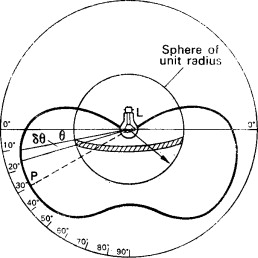
\includegraphics[width=\linewidth]{sphere2.jpg}
        \caption{Light shined over a petri dish}
        \label{fig:light-over-petri}
    \end{subfigure}%
    \begin{subfigure}{.5\textwidth}
        \centering
        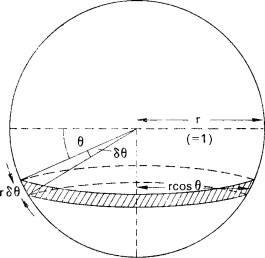
\includegraphics[width=\linewidth]{sphere.jpg}
        \caption{Light flux at different parts of a Petri dish}
        \label{fig:light-flux-petri-dish}
    \end{subfigure}
    \caption{Visualization of light interaction with a Petri dish \citep{edwards_1970}.}
\end{figure}
This means that now we can use that in the simulation to simulate the imperfections of light sources. 

Most uses a single light bulb to illuminate the Petri dish as the Petri dish is small. 

It is very important to calculate how far away the light source is from the Petri dish in order to make useful light calculations later on. This is because if the light source is very far away, the angle of incidence $\theta$ is very close to $90^\circ$, so the effect of the angle is insignificant.

In real experiments, the chemical reaction that occurs on the gel surface is sensitive to light due to the specific catalyst used (Ru(bpy)$_3$SO$_4$). 
However, to observe and record the process, they need to use light to illuminate the gel, so that the camera can capture images. The experiment design, including time-varying intervals of different light intensities, allows them to balance between controlling the reaction and capturing the activity on the gel. \cite{TOTH20091605}

They all project a single light bulb and then use a mask to have the shape they want projected, such that light does not kill off the reaction and there is light everywhere else. This is important to show how imperfections can affect the simulation . \cite{gorecki2003chemical}
An experimental setup for observing pulses in a photosensitive BZ reaction, as detailed in the work by Gorecki et al., is illustrated in the following Figure~\ref{fig:gorecki-setup}. This setup is crucial for understanding the dynamics of light-sensitive chemical reactions and their applications in computational models.

\begin{figure}[H]
    \centering
    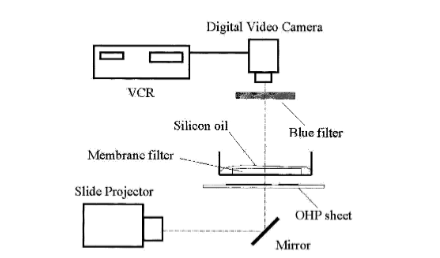
\includegraphics[width=0.7\linewidth]{images/Screenshot 2024-03-10 at 20.23.20.png}
    \caption{Experimental setup for observing pulses in a photosensitive BZ reaction \citep{gorecki2003chemical}.}
    \label{fig:gorecki-setup}
\end{figure}

\cite[71]{cui2004synchronization} contains a similar setup and goes into more detail how they project the pattern onto the gel. 
The book goes into more detail helpful for understanding the real-life environment where the waves propagate. 
One interesting observation is that the observation angle seems to change where we see the wave, which might be relevant for measuring the size of the waves, however this is not explored in this project.

\begin{tcolorbox}[colback=red!5!white,colframe=red!75!black,title=Assumption]
Unfortunately, \cite{gorecki2003chemical} do not specify how far away the light bulb projector is, which is used to illuminate the Petri dish, but we can assume the projector is far away, such that the angle of light projection is very close to $90^\circ$, making the effect of the angle insignificant. 
\end{tcolorbox}
We can still simulate that in our simulation to see what effect it would have if it were close to the medium; for larger circuits, this effect would be visible. Given a normal setup, what would be the maximum size of the Petri dish in a simulation before the effects of the light angle start to impact the simulation.




The distance between the active channel and the signal bar is 0.4 mm, which corresponds to exactly 2px in the simulation. 

Both stripes are 2 mm wide, the signal channel is 10 mm long, and the detector part is 6 mm long. The gap between the signal and the detector channels is 0.4 mm. The light intensity was selected so that the non-illuminated parts of the membrane were excitable, whereas the excitations died in the illuminated areas. In the experiment, the light intensity was set at I ) 24 kLx as determined by a light metre (ASONE LM-332), and the temperature was 295 $\pm$ 1 K \citep{gorecki2003chemical}.


From the provided information in the paper and the datasheet for the JCD100V-300W halogen bulb, we have the following data:

\begin{itemize}
    \item Luminous flux ($\Phi$) as specified in the datasheet = 6600\, $\text{lm}$ \citep{fujilamp2024jdc}
    \item Light intensity (I) at the Petri dish = 24,000\, $\text{lux}$
\end{itemize}

Originally, we calculated the luminous flux using the estimated luminous efficacy of 17 $\frac{\text{lm}}{\text{W}}$ and the power of the bulb (P) as 300 W, which gave us:
\[
\Phi_{\text{estimated}} = \text{Power of bulb} \times \text{Luminous efficacy} = 300\, \text{W} \times 17\, \frac{\text{lm}}{\text{W}} = 5100\, \text{lm}
\]
However, this was an approximation. The datasheet for the bulb specifies a luminous flux of 6600 lm, which suggests that our assumption for the luminous efficacy was incorrect.

Using the inverse square law, which relates the light intensity (I) to the distance (r) from the light source, we have:
\[
I = \frac{\Phi}{4\pi r^2}
\]
Solving for the distance (r) with the correct luminous flux, we get:
\[
r = \sqrt{\frac{\Phi}{4\pi I}}
\]
Substituting the values from the datasheet and the light intensity measurement, we find:
\[
r = \sqrt{\frac{6600\, \text{lm}}{4\pi \times 24,000\, \text{lux}}}
\]
\[
r \approx 0.148\, \text{metres}
\]

Thus, the corrected distance from the light source to the Petri dish, using the accurate luminous flux from the datasheet, is approximately 0.148 metres or 14.8 centimetres. This distance is crucial, as it suggests that the light intensity measurement of 24 kLux is likely taken close to the Petri dish where the biological samples are studied, rather than at an arbitrary point close to the light source.

\begin{figure}
    \centering
    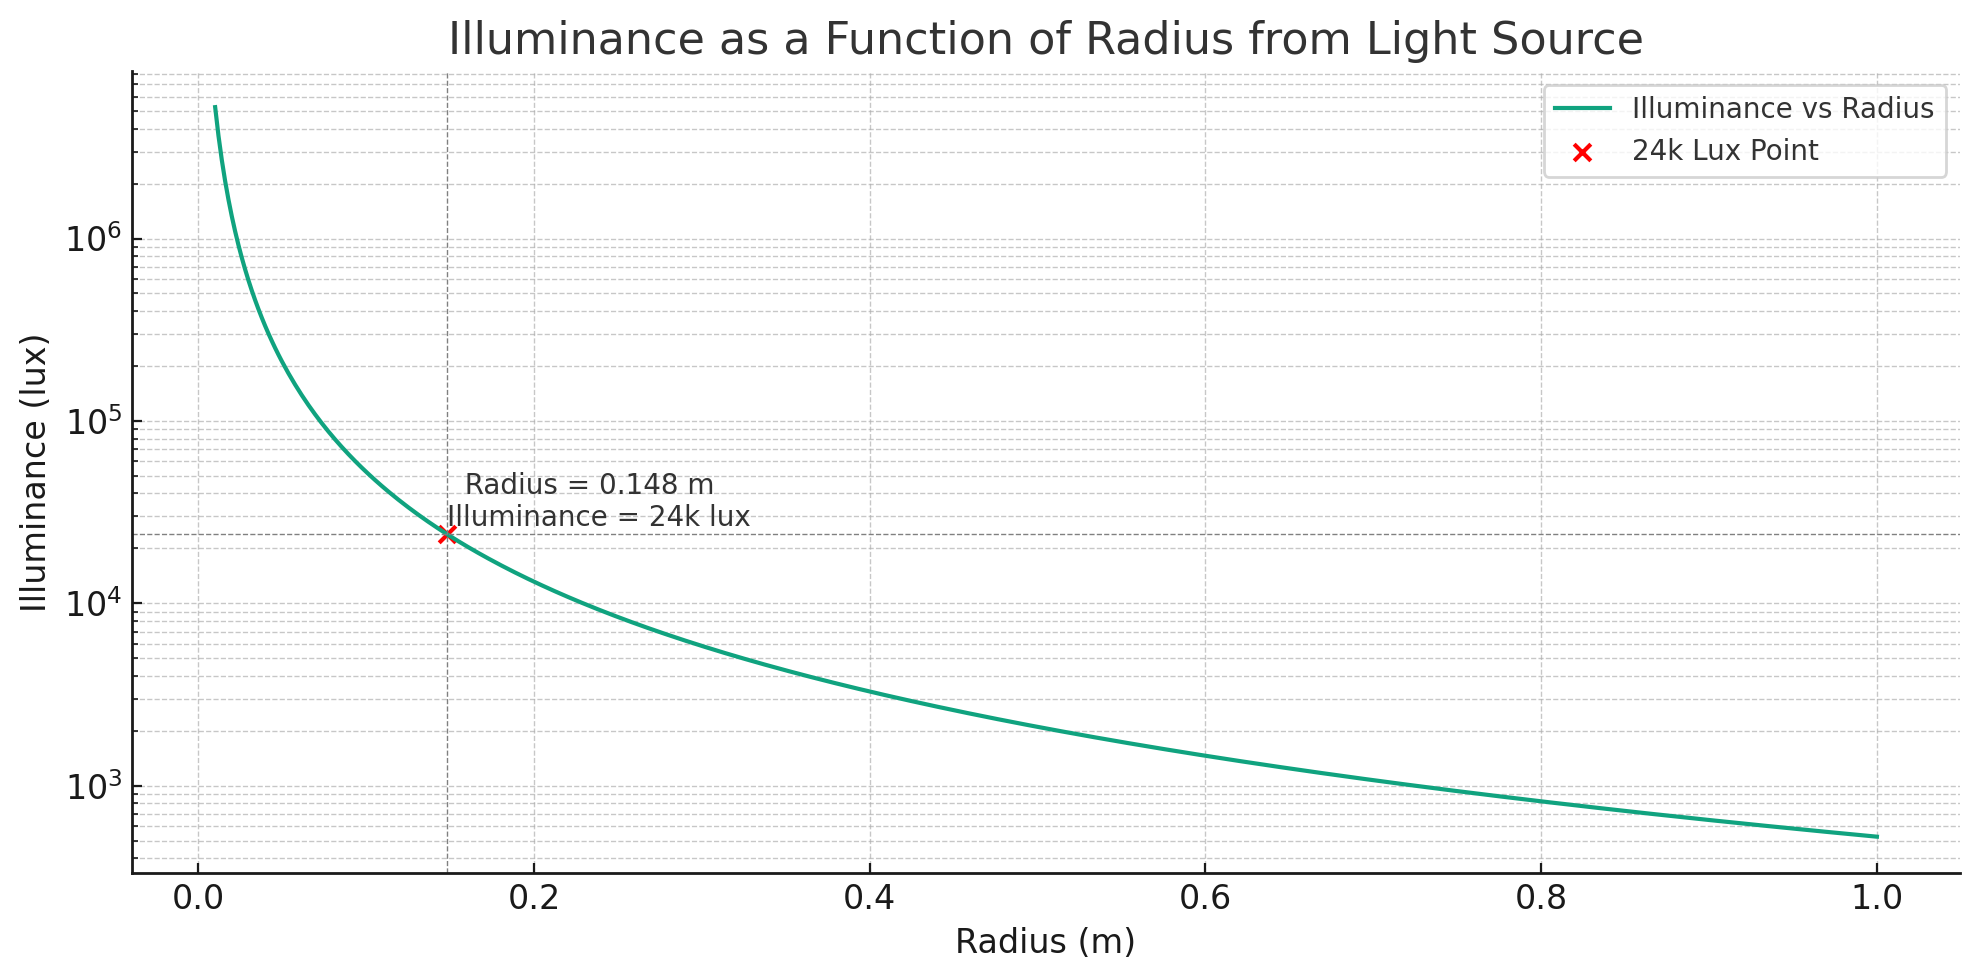
\includegraphics[width=\linewidth]{radius-illumination.jpg}
    \caption{Radius Illumination Graph}
    \label{fig:radius-illumination}
\end{figure}

In figure \ref{fig:radius-illumination} it is shown how the radius impacts the intensity at the light. 
Given the luminous flux \( \Phi \) of the JCD100V-300W bulb as 6600 lumens, we can calculate the illuminance \( I \) at various distances from the light source. The illuminance is given by the formula:
\[ I = \frac{\Phi}{4\pi d^2} \]
where \( d \) is the distance from the light source in meters.

For distances of 10 cm, 12 cm, 18 cm, and 20 cm, the illuminance values calculated are:

\begin{itemize}
    \item At 10 cm: \( I \approx 52521 \) lux
    \item At 12 cm: \( I \approx 36473 \) lux
    \item At 18 cm: \( I \approx 16210 \) lux
    \item At 20 cm: \( I \approx 13130 \) lux
\end{itemize}

These values illustrate a significant change in illumination as the radius increases, indicating that the radius is a crucial factor in determining the intensity of light received at a point.

Concluding from these calculations, it is likely that the measurement of 24 kLux was made relatively close to the Petri dish. This is because the light intensity of 24 kLux is a practical measure for the conditions under which biological samples are typically studied. Measuring illuminance right next to the light source would yield an impractically high value, which is not as useful for experimental purposes. Hence, the measurement taken is more likely to be representative of the actual working conditions near the Petri dish.


\section{Estimating The Maximum Petri Dish Size for a Chemical Diode \citep{gorecki2003chemical}} \label{sec:computer-size-limitations}


Next thing is to add the imperfection in the simulation with only an AND gate. To do that, I need to come up with a formula about plugging in a pixel and getting out the illumincation percentage. 
The percentage is basically the $\cos\theta$ as it is 0 when the angle is $90^\circ$.
let's assume a parallel light source is max intensity and an angle of 0 is no intensity at all, so in the formula we would plug in $\phi=0.054$ for when it's active and $\phi=0.0975$ when it's passive. Active means no light, passive means a lot of light, so when the light source becomes weak at a point, that would mean thath $\phi$ becomes more active. 
let's come up with a formula in mm that tells us when we move 1mm from the center of the petri dish where the light is most intense, what angle is that. That should be pretty simple, we have a right triangle, 
\begin{figure}
    \centering
    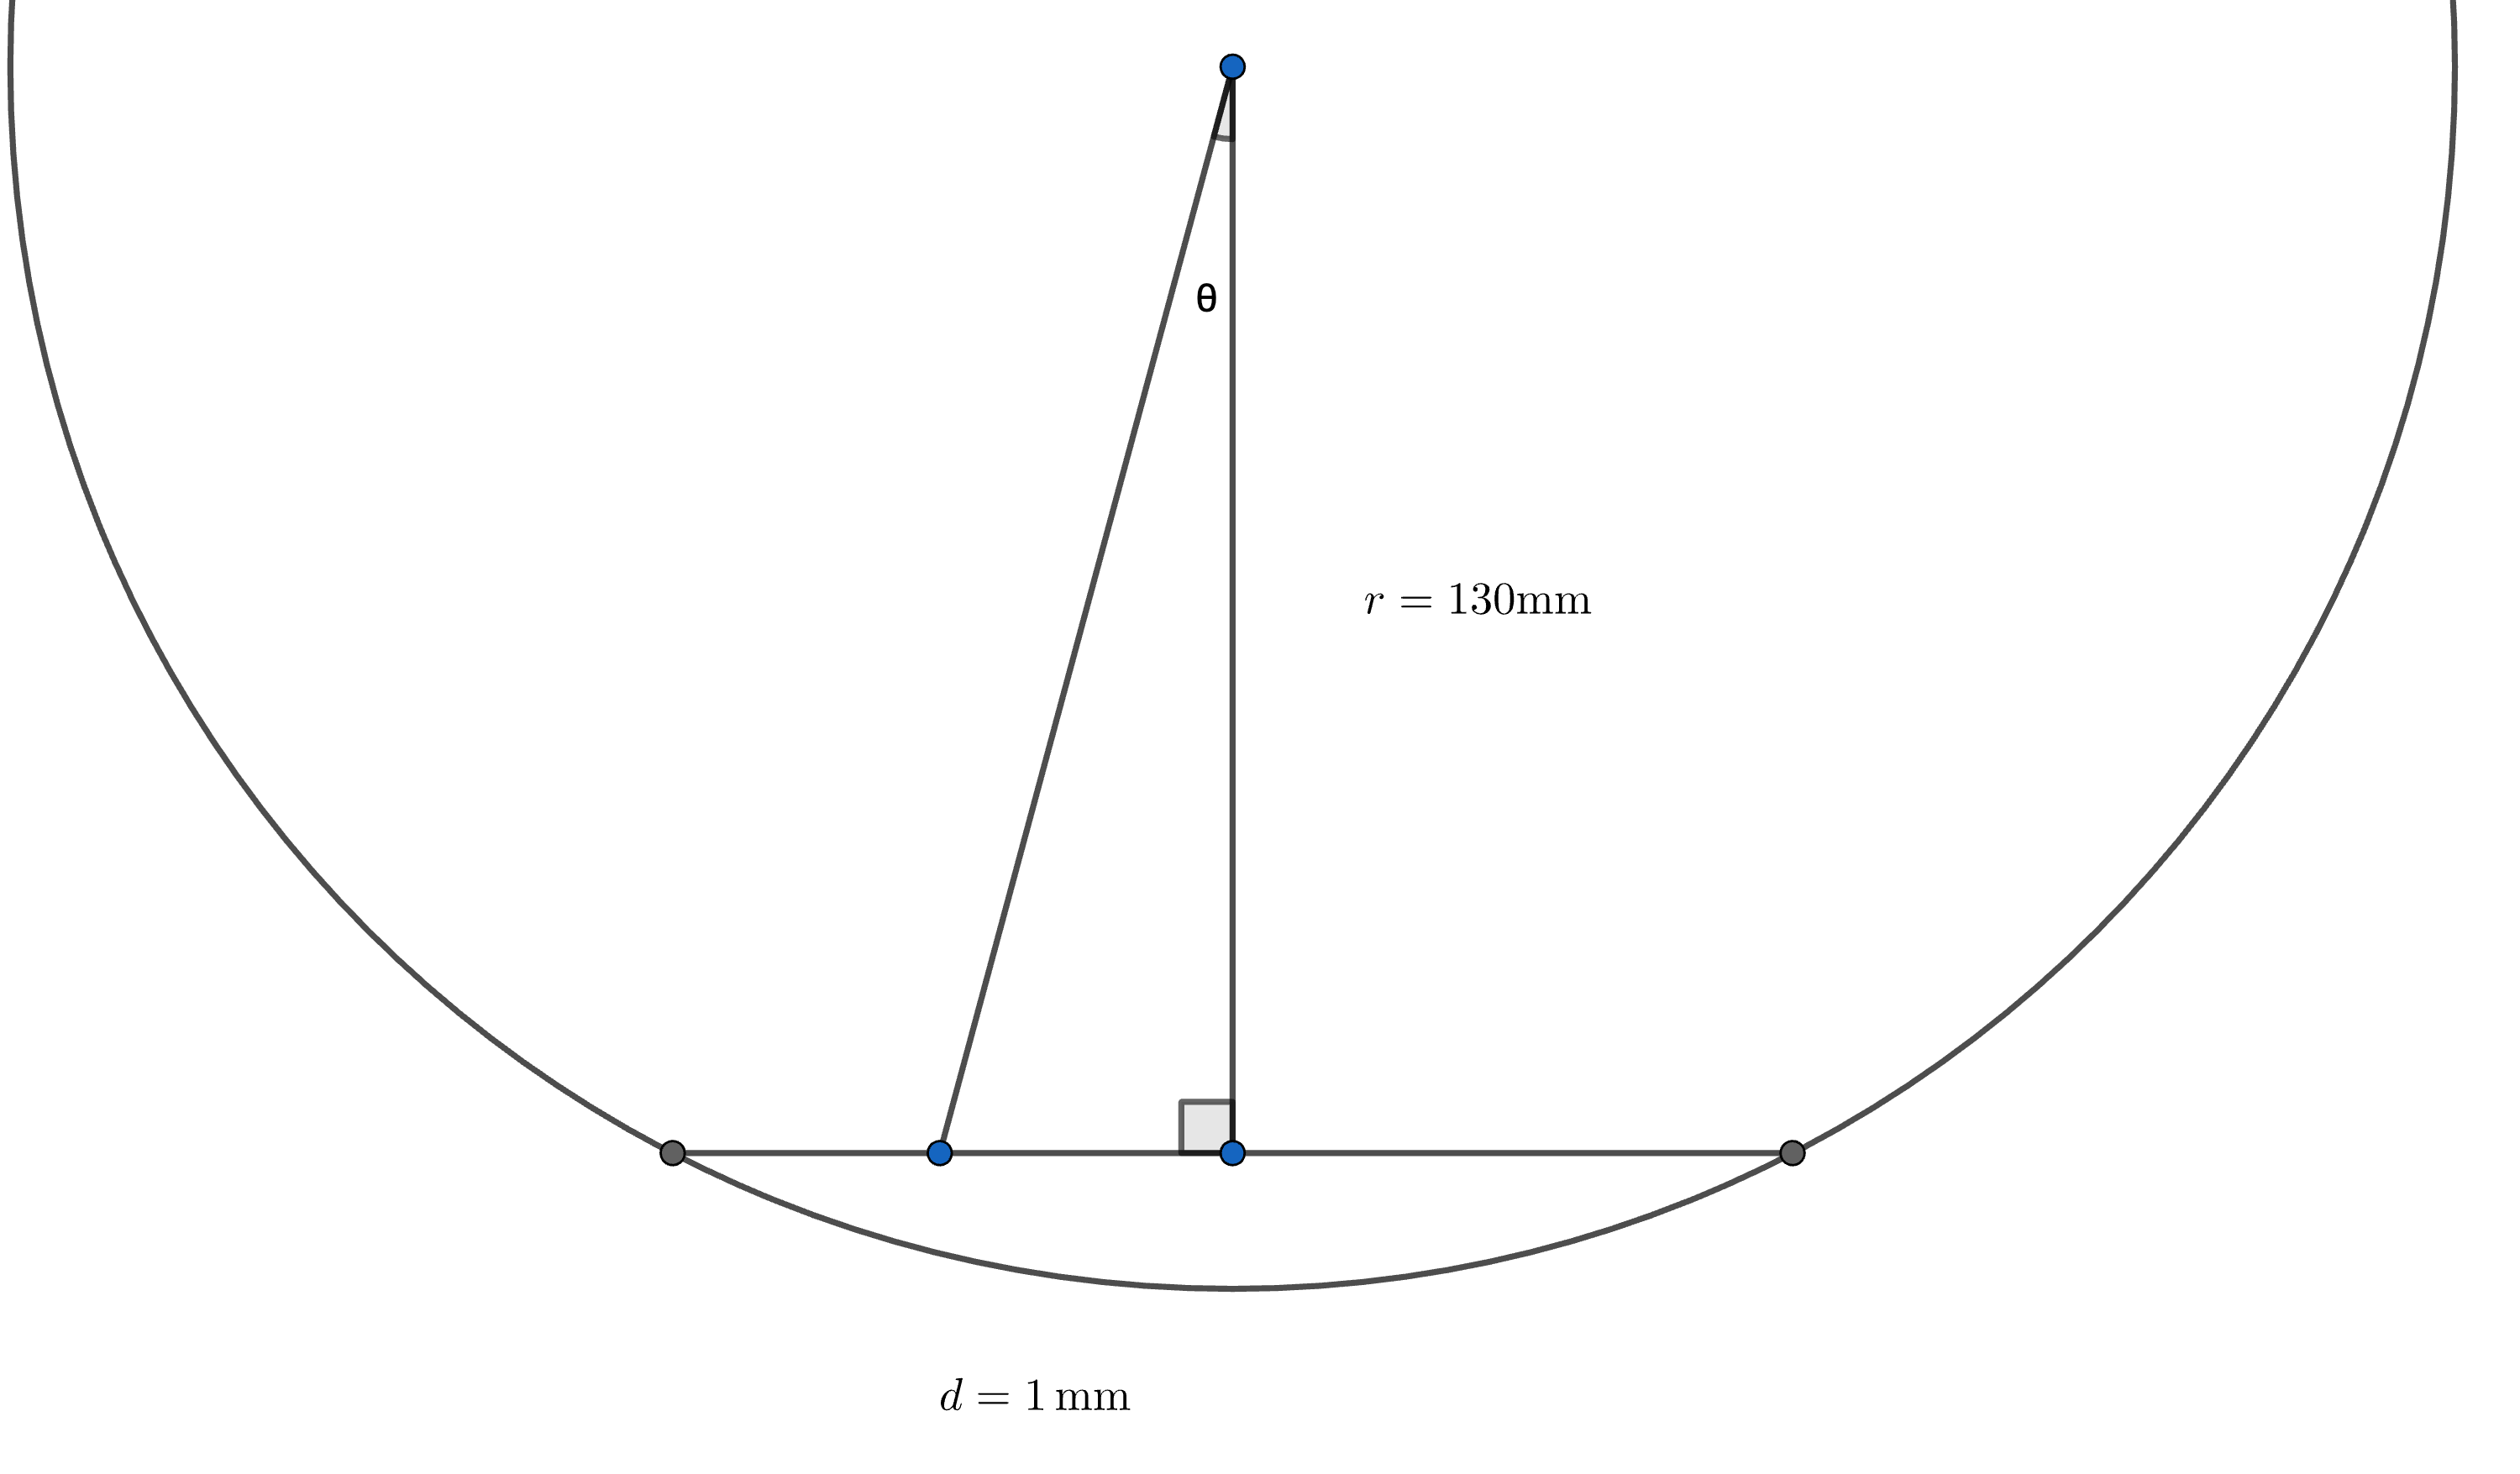
\includegraphics[width=1\linewidth]{geogebra-export (1).png}
    \caption{Illustration of finding the angle $\theta$}
    \label{fig:finding-theta}
\end{figure}

We have to find the angle every time when we move \( x \) mm from the center of the petri dish.

To calculate the angle \( \theta \) for any given radial distance \( r_c \) from the center of the Petri dish, we convert the pixel distance \( p \) to millimeters using the scaling factor \( s \) (in px/mm):

\[ r_c = p \times s \]

The angle \( \theta \) is then found using the arctangent function with respect to the height \( h \) of the light source above the center of the Petri dish:

\[ \theta = \arctan\left(\frac{r_c}{h}\right) \]

The percentage of illumination \( I_p \) at this radial distance is given by the cosine of \( \theta \):

\[ I_p = \cos(\theta) \]

Since \( \cos(\arctan(x)) \) simplifies, we can express \( I_p \) directly as:

\[ I_p = \frac{1}{\sqrt{1 + \left(\frac{r_c}{h}\right)^2}} \]

The real-world distribution of light as we get further away from the center of the Petri dish is illustrated in Figure~\ref{fig:illumination-percentage}.

\begin{figure}
    \centering
    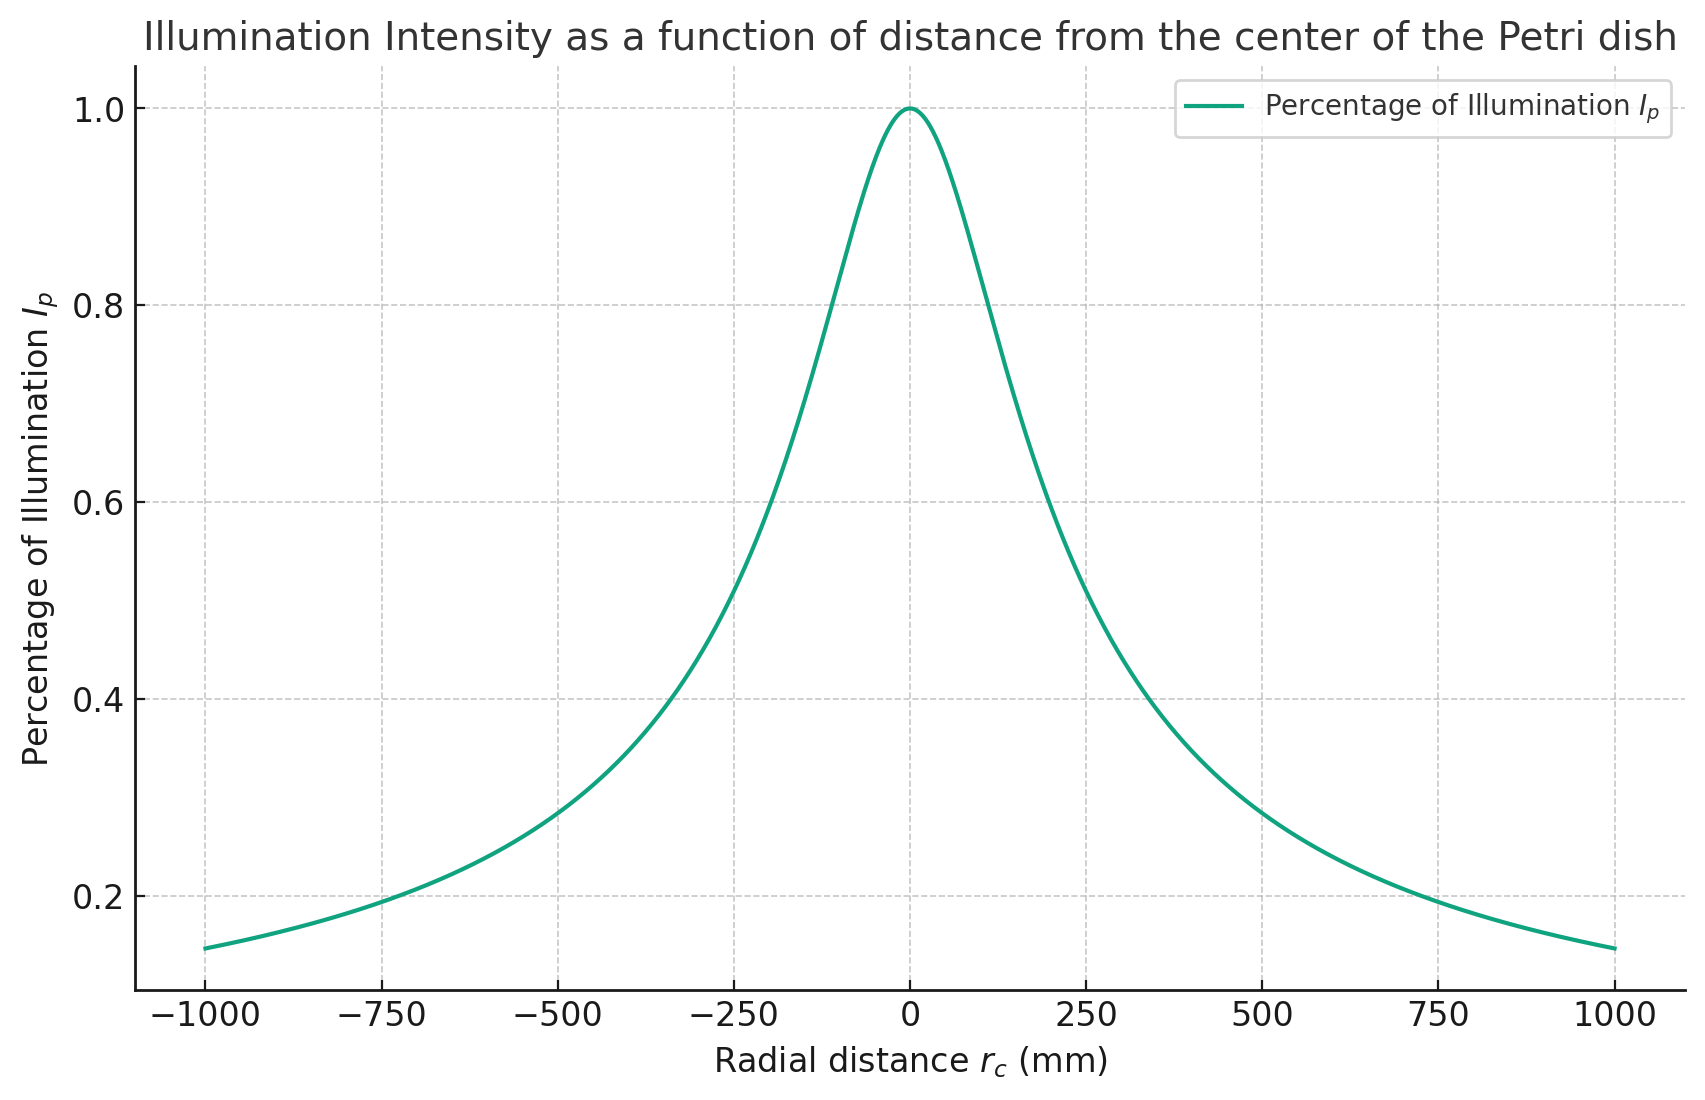
\includegraphics[width=1\linewidth]{images/831353b8-f4b4-4a93-9c41-ba3d6b6f5811.jpg}
    \caption{The graph represents the percentage of illumination $I_p$ as a function of the radial distance $r_c$ from the center of the Petri dish. The illumination percentage is calculated using the equation:$I_p = \frac{1}{\sqrt{1 + \left(\frac{r_c}{h}\right)^2}}$
    where \( r_c \) is the radial distance from the center of the Petri dish in millimeters, and \( h \) is the height of the light source above the center of the Petri dish, which is 148 mm. The graph extends from \( r_c = -1000 \) mm to \( r_c = 1000 \) mm to illustrate the symmetrical decrease in illumination intensity on both sides of the center point.}
    \label{fig:illumination-percentage}
\end{figure}



\begin{tcolorbox}[colback=red!5!white,colframe=blue!75!black,title=Assumptions for mapping light intensity to radial distance]
    In our analysis, rather than directly calculating the rate of change of distance with respect to illumination intensity (\(\frac{dl}{d\phi}\)), we employ an interpolation strategy to estimate the illumination percentage between \(\phi_{\text{active}}\) and \(\phi_{\text{passive}}\). This approach is particularly advantageous because it allows us to model the transition of the chemical diode's state from passive to active (and vice versa) without necessitating a precise mathematical mapping of the inverse square law in this context. 

    Interpolation is mathematically straightforward and significantly practical for our purposes. By defining \(\phi_{\text{active}} = 0\,\text{lux}\), representing the absence of light, and \(\phi_{\text{passive}} = 24,000\,\text{lux}\), as the maximum light intensity for the diode to remain passive, we create a linear scale between these two points. Thus, any given illumination intensity, \(\phi\), can be represented as a percentage along this scale:
    
    \[
    \text{Illumination Percentage} = \frac{\phi - \phi_{\text{active}}}{\phi_{\text{passive}} - \phi_{\text{active}}} \times 100.
    \]
    
    This formula effectively captures the transition of illumination across the operational range without delving into the complexities of the inverse square law and its derivatives. It succinctly demonstrates how illumination affects the diode's state by positioning any intermediate intensity level within a comprehensible operational range. Such an approach not only simplifies the mathematical analysis but also enhances our intuitive understanding of the system's behavior under varying light conditions.
\end{tcolorbox}
\begin{tcolorbox}[colback=red!5!white,colframe=blue!75!black,title=Assumptions for Light Intensity Calculation]
    There are assumptions to make when calculating the movable area of the Petri dish in centimeters.
\begin{itemize}
    \item The area of the Petri dish for a chemical diode is the same as the one for the coincidence detector = 10mm
    \item The limits ($\phi_{\text{min}}$ and $\phi_{\text{max}}$) are the same for both the coincidence detector and the chemical diode, in reality the coincidence detector has tighter constraints because it's made of diodes and a detector.
    \item We assume the light bulb is not using soft light, i.e. it has no piece of paper, so the inverse square law accurately describes the light intensity at different distances from the light source. 
\end{itemize}
\end{tcolorbox}

\begin{figure}[h]
    \centering
    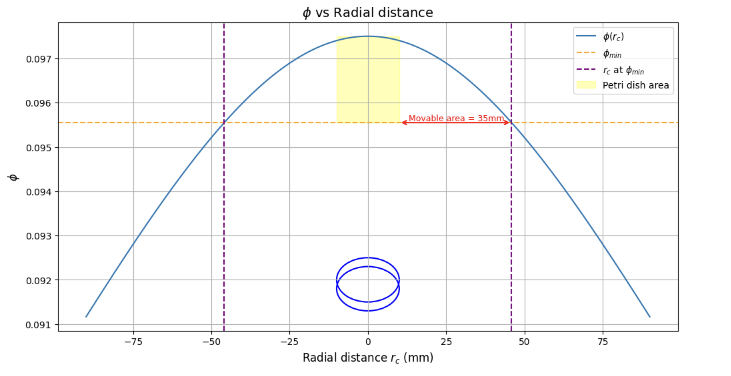
\includegraphics[width=\textwidth]{images/Screenshot 2024-03-10 at 23.57.42.png}
    \caption{The graph illustrates the illumination intensity (\( \phi \)) as a function of radial distance from the center of a Petri dish, represented by an oval at the bottom center. The shaded area within \(\pm 10\,mm\) indicates the physical size of the Petri dish. A movable area of approximately 35.87 mm from the edge of the Petri dish to the radial distance corresponding to \( \phi_{\min} \) is highlighted, demonstrating the operational range within which the chemical diode effectively inhibits the reaction. Beyond this range, the diode becomes non-operational, allowing the reaction to proceed unimpeded.}
    \label{fig:petri-dish-illumination}
\end{figure}

In this analysis, \( \phi_{\text{passive}} \) is defined as the maximum illumination intensity under which the Belousov-Zhabotinsky (BZ) reaction-based chemical diode remains in a passive state, effectively inhibiting the chemical reaction from propagating. The diode operates within this passive state until the illumination intensity decreases to a critical threshold, \( \phi_{\min} = 0.09555 \). Below this threshold, the diode becomes non-operational and ceases to inhibit the reaction, allowing it to propagate freely. The state of no light, denoted as \( \phi_{\text{active}} \), represents an ideal condition that is not physically achieved in this setup but is simulated using a filter to create the circuit pattern. \( \phi_{\min} \) was chosen based on experimental configurations and literature by Gorecki et al., signifying the operational limit for the diode's passive behavior. This analysis emphasizes the transition from \( \phi_{\text{passive}} \) to a non-operational state as light intensity falls below \( \phi_{\min} \), underscoring the critical operational range for the chemical diode's function in the BZ reaction.



\section{Light Impact on a CMM Neuron \citep{stovold2017reaction}} \label{sec:light-impact-cmm-neuron}
This formula calculates the percentage of illumination at a point \( r_c \) millimeters from the center, assuming the light intensity directly beneath the source is 100%.
\todo{This here is related to the big circuit that James has, not the and gate or the diode}


From manual tests with illumination, the circuits start behaving not as expected even with illumination percentages less than 0.99 because the simulation is very sensitive to changes in light intensity as it relies on a manifold of light-affected microinteraction. Using this value of 0.99, we can see at what size of the Petri dish do we start to see values below 0.99. We can calculate that and then confirm in the simulation. 


I debugged the nonworking thing with a debug variable inside the metal function controlled by my mouse. 
I just verified that the simulation does break once the illumination reaches 0.99. I did not get much value from putting this inside the simulation, more like, oh yeah, I am correct.
I could have verified that 0.99 is the threshold by just running 
it.

I verify using a simulation that if the circuit is too big, a single light source might not be enough to illuminate the whole area relatively evenly and even light perturbations in the light are going to disrupt larger circuits. 
What can be done is to make the circuit different the further away it is from the source, which would involve different dynamics that work under different lighting conditions. This is infeasible to do practically as it so highly depends on the light source. 

The 0.99 is kind of sus, I still need to figure out a lot of things like a more optimal mapping from the real-life illumination intensity and the mathematical formula in the Oregonator model. I think my mapping is okay because $\phi_{\text{active}}$ is what it is and $\phi_{\text{passive}}$ can be moved even further, I just interpolate between these values, maybe there is a better way to simulate it. The problem with my simulation is that it does not matter how strong the light source is, you can put the whole sun over the Petri dish, the illumination at the angle is still going to be 0.99 of the original, I need a better way to simulate it that can also input the parameters of the light source, so it's not just about the strength. I need something like a threshold for when the light intensity is so strong that nothing can pass through. That is also a problem, however, because the actual circuit relies on the gaps being not too illuminated, so that the activator chemical can diffuse towards another part of the surface. It's again difficult to come up with a model. 
So that means a more powerful light bulb might create different things for different illuminations, but it might not work if the Petri dish is directly under it as it might create too much illumination and prevent the waves from crossing boundaries. \textit{I don't know}. So the 0.99 is only true when the assumption that $\phi_{\text{active}}$ is equivalent to the Hallogen light bulb of 300W used directly above it.

Maybe, just maybe, the relationship is not linear as I assume, but logarithmic, so as the illlumination in real life decreases, that creates a logarithmic decrease in $\phi$ from $\phi_{\text{active}}$ to $\phi_{\text{passive}}$, so it might not be as sensitive to the small changes in light as I assume. \todo{To resolve this, how did the var values come about }

In the simulation very small changes in light intensity were found to very significantly affect the propagation delay of the activator signal. This is crucial for the operation of the circuit. These circuits do not have any way of synchronisation other than propagation delay, which means even the slightest change in light intensity is going to affect the speed of propagation and the whole circuit would break. This is more important for bigger circuits like the ones built by \cite{StovoldJames2019RaGI}, that rely heavily on exact propagation. 
In my simulation it was very sensitive to the illumination changes, maybe in real life as long as it's more illuminated than some \textit{threshold}, then it doesn't matter for the simulation. I need to do more digging to figure out what to do from here.






Ok, I need to understand how illumination maps to $\phi$. For that I need to understand the Oregonator model


that's it, we need to find the minimum and maximum reaction rates in real life reactions. 
we already have a minimum and maximum in the simulation ,we can check if they behave the same way. if they do, that's our threasholds, then we need to find an appropriate function that describes a similar relationship and we found it


The main idea is that when there is no activator in the solution,  \citep{reddy1995effect}






% Always start your chapter on a new page!


%%
%% You bib file
%%
\newpage
\bibliography{report}

\newpage
\appendix
%%
%% Your appendices
%%
\chapter{Creating a Coincidence Detector In Simulation} \label{chap:creating-detector}
Developing the AND gate posed a significant challenge as it is highly dependent on specific geometric configurations for proper operation. 
While it is acknowledged that such a coincidence detector is feasible, the focus of our investigation is on the stability of such simulations in response to environmental changes and the practicality of implementing them in a real environment.
Although we acknowledge that building this in a simulation is possible, the focus of this paper is to determine the stability of the simulation in response to environmental changes and the practicality of implementing them in a real environment. 


\section{Unsuccessful Detector}\label{unsuccessful-detector}
\begin{figure}
    \centering
    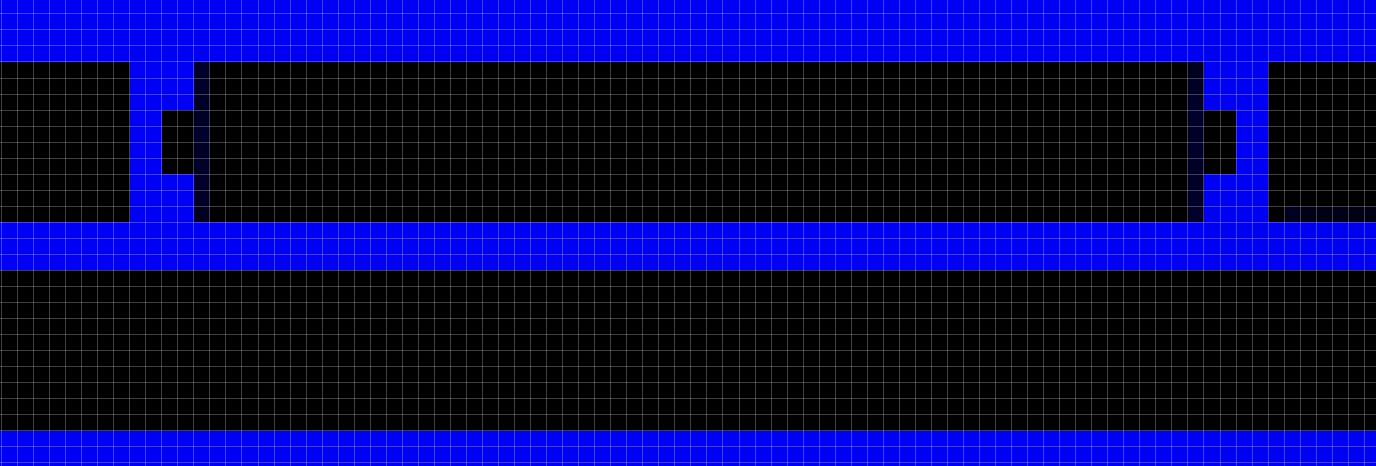
\includegraphics[width=0.75\linewidth]{image7.png}
    \caption{Initial Coincidence Detector Configuration}
    \label{fig:unsuccessful-config-and-gate}
\end{figure}
\begin{table}[h]
\centering
\begin{tabular}{|c|c|c|c|c|}
\hline
Width & Gap=1px & Gap=2px & Gap=3px & Gap=4px \\ \hline
w=1px & NP & NP & NP & NP \\ \hline
w=2px & NP & NP & NP & NP \\ \hline
w=3px & AP & NP & NP & NP \\ \hline
w=4px & AP & AP & NP & NP \\ \hline
w=5px & AP & AP & NP & NP \\ \hline
w=6px & AP & AP & NP & NP \\ \hline
w=7px & AP & AP & NP & NP \\ \hline
w=8px & AP & AP & NP & NP \\ \hline
w=9px & AP & AP & NP & NP \\ \hline
w=11px & AP & AP & NP & NP \\ \hline
w=12px & AP & AP & NP & NP \\ \hline
w=13px & AP & AP & NP & NP \\ \hline
\end{tabular}
\caption{Results of the experiment showing the relationship between conductor width and gap size.}
\label{table:experiment-results}
\end{table}
In our investigation, we focus on three controllable variables: 
\begin{itemize}
    \item the width of the conductor
    \item its length before the gap.
\end{itemize}
The detector configuration is shown in Figure \ref{fig:unsuccessful-config-and-gate}.
The primary question we seek to answer is how the width of the conductor influences the functionality of the gates. Specifically, our experiment aims to identify an optimal conductor width that enables the "if" gate to function correctly. This gate's operation relies on two conductors positioned closely, requiring a precise amount of force to facilitate signal transmission from one to the other. This force is generated by the collision of two waves. However, current configurations fail due to the conductors being excessively proximate.

For the purposes of this experiment, we define three outcomes based on the interaction between the waves and the conductors:
- Always pass (AP): The signal always passes through the gap.
- Never pass (NP): The signal never passes through the gap.
- Collision pass (CP): The signal passes through the gap only upon collision of waves.

The CP outcome is of particular interest as it represents the desired state for computational functionality.

Initial tests did not yield CP outcomes, suggesting a potential discrepancy in the values of $\phi_{active}$ versus $\phi_{passive}$. Adjusting $\phi_{active}$ to a more aggressive value of 0.035f resulted in CP outcomes for every gap of 3px, marking a significant deviation from the default value of 0.054 proposed in prior literature. This finding prompts further investigation into the range of values between 0.035 and 0.054 to identify a flexible operational window. 

A successful configuration identified involves a long charge, a gap of 3px, and a $\phi_{active}$ value of 0.035. Further exploration is required to determine a viable configuration for a gap of 2px.

Additionally, our observations reveal notable differences in wave behavior depending on orientation; specifically, vertical wave propagation exhibits distinct properties compared to horizontal propagation. A particularly intriguing observation is that waves originating off-center tend to accelerate asymmetrically, favoring one direction over the other, and resulting in a higher likelihood of collision.

\section{Successful Detector}

Section \ref{unsuccessful-detector} led to the conclusion that there must be more parameters in play that prevent the detector from functioning, and it was later found that the height of the diode pin on the active medium of the coincidence detector. 
Following this, it was discovered that by setting the pins higher or lower, we change from where the wave approaches the detector medium, allowing for a finer adjustment of the opration. This created the first successful detector, seen in Figure \ref{fig:first-successful-detector}.

\begin{figure}
    \centering
    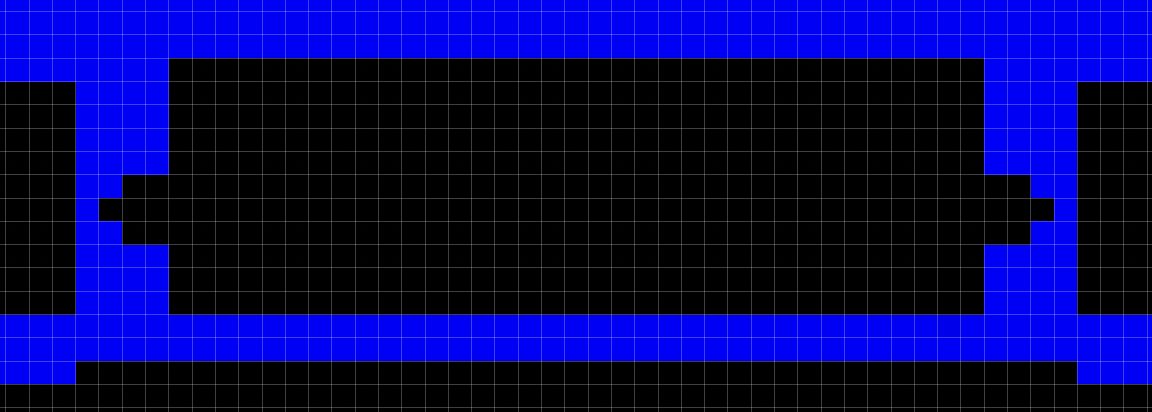
\includegraphics[width=0.75\linewidth]{image9.png}
    \caption{First Successful Coincidence Detector}
    \label{fig:first-successful-detector}
\end{figure}


Normally the wave also depends on where it is coming from, but we can ignore that in our case because we are using diodes at entry of the detector medium. Diodes add a new entry point for the incoming wave, so the incoming direction does not really matter. 

There is still a small problem with this design where if two waves meet around the centre, none of them gets enough momentum to develop fully and they don't have enough concentration to diffuse into the result substrate, this can be solved by increasing the length of the detector medium to allow for both waves to form, so later designs have a longer detector medium, like in Figure \ref{fig:and-gate}

The length of the coincidence detector depends on two factors:
\begin{enumerate}
    \item The minimum distance apart they need to be from each other while still allowing for the waves to form inside the detector.
    \item The minimum distance apart they have to be, so that the centre is still usable for collusion.
\end{enumerate}
\newpage

\chapter{Original Project Proposal}
\label{chap:A1}




\section{Aims \& Objectives}
\subsection{Aims}

The aim of the project is to create one of these BZ simulations and add a number of imperfections, measuring how they impact the simulation. These imperfections would typically be found in the real world in the form of dust particles, terrain obstacles or other environmental factors.
\begin{figure}
    \centering
    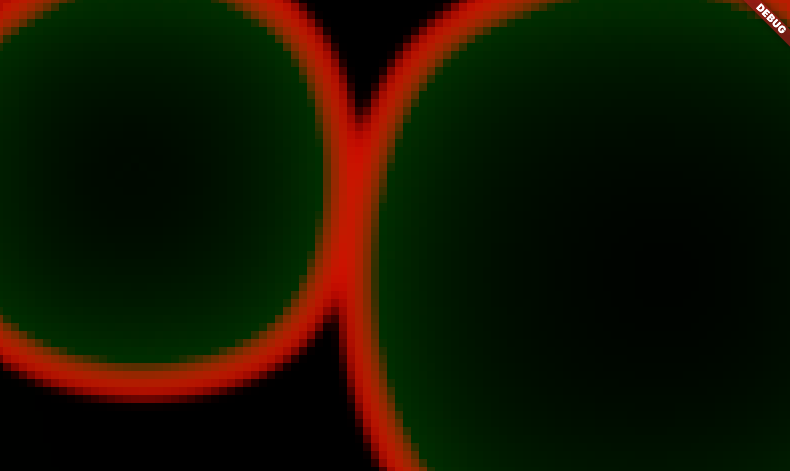
\includegraphics[width=0.75\linewidth]{original_proposal/Screenshot 2023-10-24 at 08.09.52.png}
    \caption{Expanding wave pattern from this project using the Oregonator model}
    \label{fig:first-waves}
\end{figure}

The main idea is to create an application using Flutter and to simulate the reaction. 
\begin{enumerate}
    \item Interactive Simulation App Development with Flutter
    Flutter is a mobile application framework that allows for easy addition of elements of interactivity and allows for lower level control over pixels, which is necessary for creating one of these simulations. The reason for choosing Flutter as opposed to another framework or solution is because of the already present familiarity with the framework. 

    The simulation shall run on the GPU, so addressing the GPU usage is crucial. The current solutions are to use the recently added \verb|flutter_gpu| package or integrating Dart Foreign Function Interface (FFI) to run native shaders. 
    \item Creating a game from the simulation. Since the project is focused around imperfections, it could be possible to let the user play with or against the waves (see figure \ref{fig:enter-label}) using the \verb|flame| package (minimal game engine). 

    The simulation has illumination that creates a path, the aim is to create a game where the user has to run away from the waves, but is also constrained to the illuminated area, so for example a single wave could split and then catch the player from both directions. 

    \item Adding imperfections:
    One of the main themes of the project is finding imperfections. The goal is to let the player defend himself from the waves using imperfections in the simulation that impact the reaction-diffusion model. This could mean throwing dust particles at the wave or adding temperature to the model that speeds up or slows down the reaction at a particular zone, so that a part of the waves travels more slowly, disrupting the reaction. The aim is to allow the user to only use imperfections as a means of defence. 
\end{enumerate}

\subsection{Challenges}
Among the challenges I might face I see myself running into a computational problem where dt, being as small as it is, could force me to run the simulation at a very slow rate, which then would make me increase the speed at which it is run, using more CPU, but since the project is \textit{real time}, I cannot afford to go beyond the maximum allowed CPU per frame or I would cause jitter, running code on the GPU should help, but there also needs to be a way to only perform these calculations on a subset of the whole map. Also if this were a game, there could be beacons generating these waves that the user has to destroy. Flutter also has a 2D game engine that I've wanted to explore and that could be a great opportunity. 
The other reaction-diffusion systems are very scientific or are presented as a video. \cite{doi:10.1021/jp509474w} have used reaction and diffusion to find the shortest path in a maze. 

\section{Related work}
The area of reaction-diffusion simulations has been explored well. The simulations of waves are used to produce computing units like counters and logic gates \citep{gorecki2003chemical} as well as neurons \citep{StovoldJames2019RaGI}. 

\cite{edge2020chaotic} has created a game (figure \ref{fig:chaotic-edge-game}) out of the Gray-Scott model where ships battle inside of a goo-like substance and the chemical acts as a dynamic obstacle. The game looks of very high quality despite the lack of interest from the public. Other than this project, there isn't a lot of interest in the joint field of reaction-diffusion simulations and gaming
\begin{figure}
    \centering
    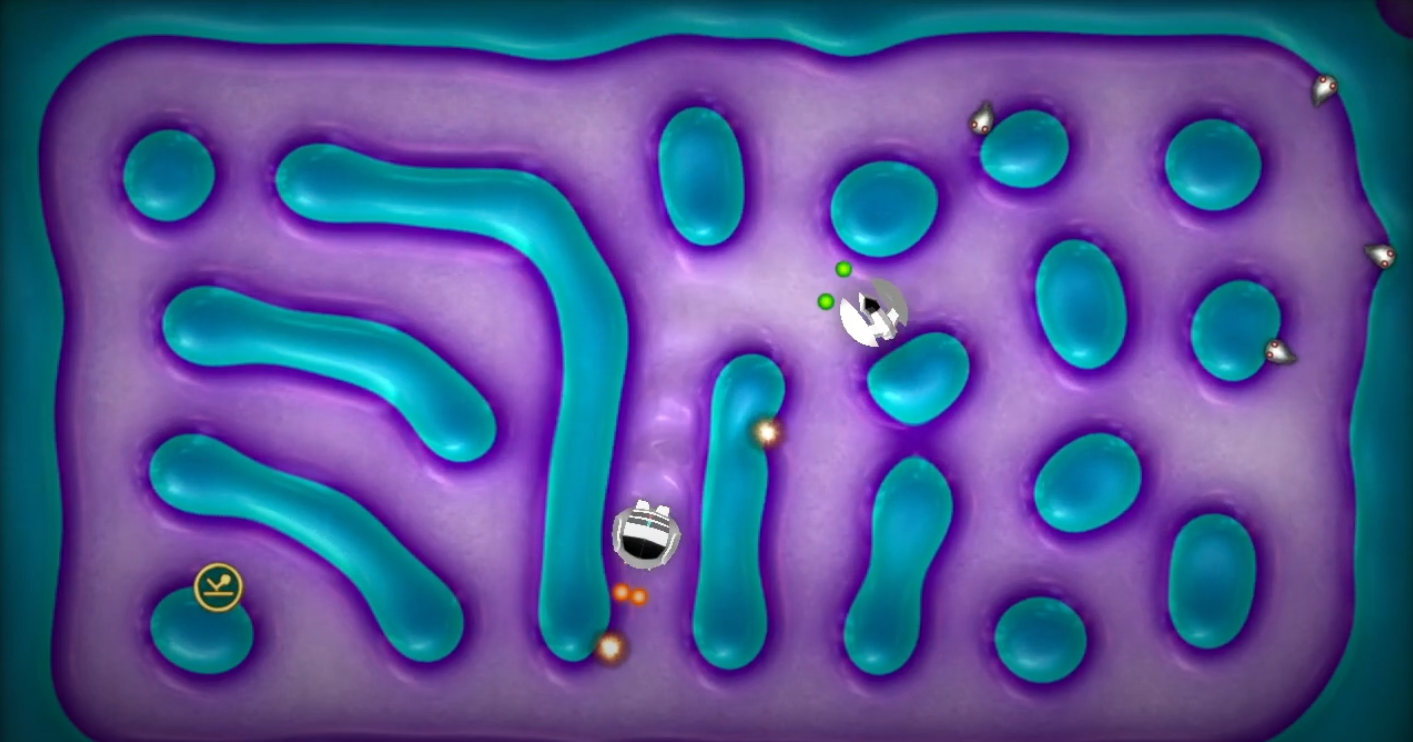
\includegraphics[width=0.75\linewidth]{original_proposal/Screenshot 2023-10-26 at 06.06.23 (1).png}
    \caption{Reaction Diffusion Game by Chaotic Edge}
    \label{fig:chaotic-edge-game}
\end{figure}
\section{Methodologies}
\begin{enumerate}
    \item The project is going to use an agile iterative approach where the phases of the Software Development Life Cycle are performed every sprint.

    \item It's important is that the work is broken down into chunks according to the SMART task framework, which stands for Specific, Manageable, Achievable, Relevant, Time-bound. It's important for the tasks to be small and understandable, without any dependencies to other tasks
    \item If one task requires the parallel completion of another task, then these tasks should be the same task with two things to do in the task. 
    \item The project is going to use ClickUp as a Project Managemenet System (PMS) due to its flexibility and integration with calendar and task management apps. 
    \item The most important task management tool to be used in this project is Reclaim.AI, which uses priorities and deadlines to auto schedule your calendar based on your preferences and hours, it has an integration with the most popular PMSs like Jira, ClickUp, Asana, etc. 
    \item The Project Management System tasks are going to use custom statuses:
    \begin{enumerate}
        \item TODO - feature not started
        \item RESEARCHING - gathering information and reading about feature
        \item SUBTASKING - feature clear. creating subtasks and checklists to make task execution easier
        \item IMPLEMENTING - implementing feature
        \item TO PRESENT - feature implemented. Waiting to be presented to supervisor
        \item FOR REVISION - supervisor left feedback. Return task to RESEARCHING or IMPLEMENTING
    \end{enumerate}
    \item The project is going to use the 1 week sprints to divide work into even blocks of work if the backlog ends up being too big. If the backlog remains small , the project is going to use the backlog and not use sprints. 
\end{enumerate}
\section{Programme of Work}
The project, being agile, doesn't have strong formal phases, it follows an iterative approach. 
There are however distinct phases in the planned development of this project (see figure \ref{fig:gantt}):

\begin{enumerate}
    \item Planning \& Analysis - this phase is going to specify goals of the sprint
    \item Design - The project is going to be designed in more detail, that includes library choices, design choices, etc
    \item Implementation - This phase would take up the majority of the sprint time
    \item Testing - last phase before the project transitions into a finalising state
    \item Searching for Participants - a stage where about 5 people need to be recruited to perform evaluation
    \item Conduct evaluation - the evaluation is going to be performed using heuristics, for example how intuitive the game is, etc. 
    \item Focus on dissertation - time to shift focus on using the resources and documentation to create the dissertation.
\end{enumerate}
This project is prototypical, so it's going to have reduced planning and design phases. 
\begin{figure}
    \centering
    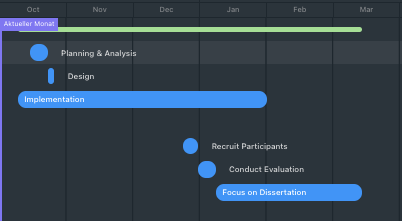
\includegraphics[width=1\linewidth]{original_proposal/Screenshot 2023-10-26 at 18.26.29.png}
    \caption{Gantt Chart}
    \label{fig:gantt}
\end{figure}

\newpage

\chapter{Another Appendix Chapter}
\label{chap:A2}

This could be about your experiments

\end{document}
